\chapter{Optimizing Machine Learning Applications Using Approximate Computing Techniques}
\label{ch:ch2}

\section{Overview}

OpenVINO is designed with the objective to accelerate machine learning applications that use CNNs. The Myriad X VPU is tailored to accelerate vision applications, so it is also optimized to run CNNs. In this chapter, three applications are tested and a set of optimization techniques are explored to find how these applications can be run faster without hurting significantly the accuracy of the results. Three classification applications were selected for testing. The first one is audio classification, the data set consists of audio files with recordings of spoken digits. The second application is fruit classification with 131 different fruit categories. The third application consists of identifying different landscape scenes such as forests, buildings, mountains and others.

The next section describes the details of the selected machine learning applications that are tested. Table \ref{tab:app_summary} show the summary of the data-sets used in the applications. After that, the description of the details of the selected topologies for each application are presented. The methodology details are shared in the following sections: the selected approximate computing optimization techniques that are implemented and the different parameters that are measured when running the applications.

\section{Applications}

\begin{table}[thbp]
\centering
\caption{Applications Summary}
\label{tab:app_summary}
\begin{tabular}{|l|l|l|l|l|l|}
\hline
\multicolumn{1}{|c|}{\multirow{2}{*}{\textbf{Application}}} & \multicolumn{1}{c|}{\multirow{2}{*}{\textbf{Categories}}} & \multicolumn{3}{c|}{\textbf{Dataset Split}}                                                       & \multicolumn{1}{c|}{\multirow{2}{*}{\textbf{Size}}} \\ \cline{3-5}
\multicolumn{1}{|c|}{}                             & \multicolumn{1}{c|}{}                            & \multicolumn{1}{c|}{\textbf{Train}} & \multicolumn{1}{c|}{\textbf{Validation}} & \multicolumn{1}{c|}{\textbf{Test}} & \multicolumn{1}{c|}{}                      \\ \hline
Audio                                              & 10                                               & 2160                       & 240                             & 600                       & 64x64x1                                    \\ \hline
Fruit                                              & 131                                              & 50769                      & 16923                           & 22688                     & 100x100x3                                  \\ \hline
Scene                                              & 6                                                & 11929                      & 2105                            & 3000                      & 150x150x3                                  \\ \hline
\end{tabular}
\end{table}

\subsection{Audio Classification}

For this application the objective is to try to identify spoken digits. The dataset used is the Free Spoken Digit Dataset \cite{fsdd}. This dataset consists of 10 classes: all the digits from zero to nine. It is composed of 3000 recordings from 6 different speakers with different accents, this means that for each digit there are 50 recordings per speaker. The dataset itself is made from wav files. These wav files are converted to spectrograms before being used. This makes the classification process easier since now the dataset is in a 2D format which can be fed to a traditional 2D CNN and the problem can be treated in the same way as a image classification problem. The resulting spectrogram has the following properties: the \textit{x} axis represents time, the \textit{y} axis represents the frequency, and the pixel intensity, in gray-scale representation, represents the amplitude of a specific frequency at a given time (see Figure \ref{fig:specs}).

\begin{figure}[thbp]
	\centering
	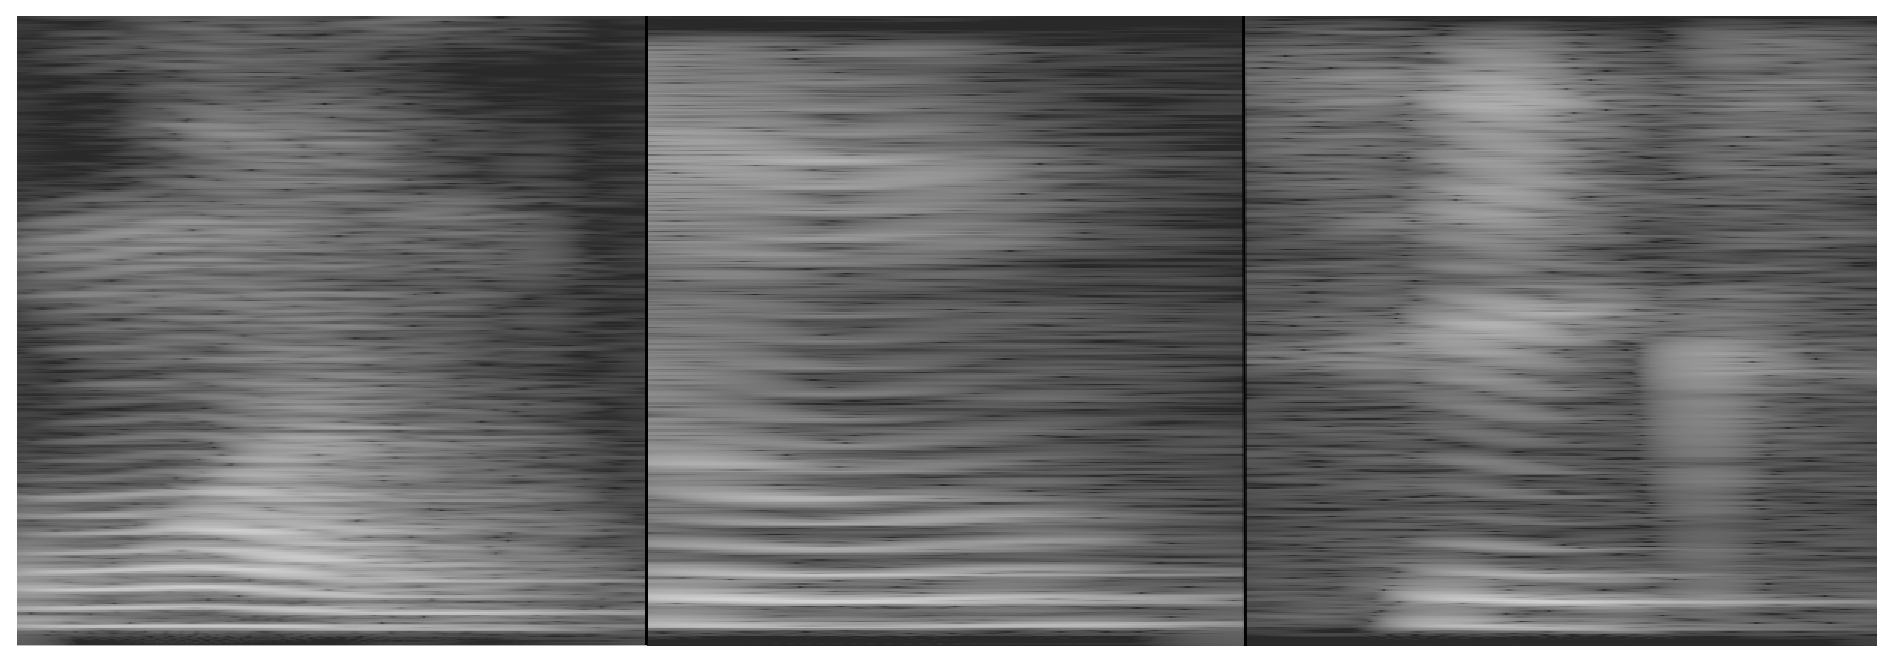
\includegraphics[scale=0.25]{specs}
	\caption{Spectrogram examples. Generated from audio files from the Free Spoken Digit Dataset \cite{fsdd}.}
	\label{fig:specs}
\end{figure}

\subsection{Fruit Classification}

This application classifies images of different types of fruits. The dataset is the Fruit Images Dataset \cite{fruit_ds}. This dataset contains a total of 90380 color images divided in 131 categories, where each category is a different kind of fruit. Each image is 100 by 100 pixels image. Figure \ref{fig:fruits} shows three examples of different fruit images from the dataset: blueberry, lime and strawberry.

\begin{figure}[thbp]
	\centering
	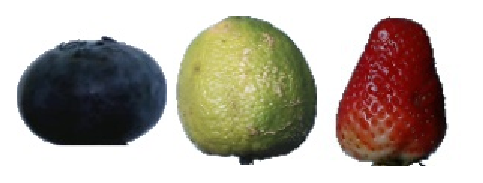
\includegraphics[scale=1.0]{fruits}
	\caption{Fruit examples. Taken from the Fruit Images Dataset \cite{fruit_ds}.}
	\label{fig:fruits}
\end{figure}

\subsection{Scene Classification}

These application classifies images of different natural scenes from around the world. The dataset is the Intel Image Classification \cite{intel_ds}. The dataset has 17034 color images of a size of 150 by 150 pixels. The categories are the following: buildings, forest, glacier, mountain, sea, street. Figure \ref{fig:scenes} shows three examples of different scene images from the dataset: buildings, mountain and sea.

\begin{figure}[thbp]
	\centering
	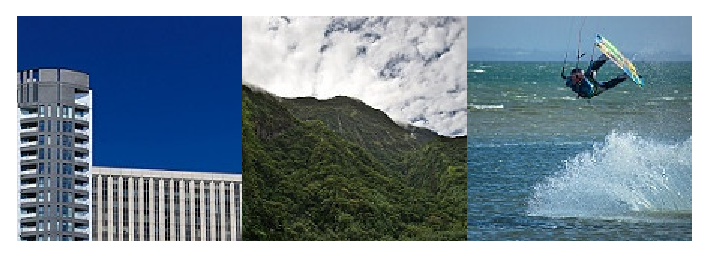
\includegraphics[scale=0.75]{scenes}
	\caption{Scenes examples. Taken from the Intel Image Classification Dataset \cite{intel_ds}.}
	\label{fig:scenes}
\end{figure}

\section{Neural Network Topologies}

Each application was trained on a different neural network, the amount of layers and the size and depth of these layers vary depending on the complexity of the application. Nonetheless, since all three applications are image classification problems they all follow a similar structure. The first layers are a convolutional layers combined with max pooling layers, which downsample the image. The pool size for all the pooling layers is 2 by 2 pixels, which means that the image is reduced to half the size. After that, there is a flattening layer which transforms the 2D image to a one-dimensional array. Finally, the network has a few dense (fully connected) layers. In the middle of the dense layers dropout layers can be inserted, which can help with overfitting. All the applications have a dropout rate of 0.25 which is a fairly typical value to use. All applications were trained for 50 epochs. The training parameters and the network topologies were chosen by trial and error in an iterative process where the parameters and topologies were refined until an optimal point was found where the size of the network was small enough and the accuracy was acceptable. Bigger network sizes had diminishing returns in accuracy for the audio and fruit classification problems. The scene classification problem still has room to improve in terms of accuracy, but for the purposes of this work an accuracy of more than 80\% was good enough and since it is the bigger network, training time was also a concern.
%Tables \ref{tab:audio_nn_topo}, \ref{tab:fruit_nn_topo} and \ref{tab:scene_nn_topo} show the topology for each of the different applications along with the total number of trainable parameters in the neural network. All applications were trained for 50 epochs.

\begin{table}[thbp]
\centering
\caption{Neural network topology for audio classification.}
\label{tab:audio_nn_topo}
\begin{tabular}{|l|l|}
\hline
\multicolumn{1}{|c|}{\textbf{Layer}}          & \multicolumn{1}{|c|}{\textbf{Details}}                     \\ \hline
Input          & shape=64x64x1               \\ \hline
Conv2D         & shape=64x64x32, kernel=3x3  \\ \hline
Conv2D         & shape=64x64x32, kernel=3x3  \\ \hline
MaxPooling2D   & pool\_size=2x2              \\ \hline
Conv2D         & shape=32x32x16, kernel=3x3  \\ \hline
Conv2D         & shape=32x32x16, kernel=3x3  \\ \hline
MaxPooling2D   & pool\_size=2x2              \\ \hline
Flatten        &                             \\ \hline
Dropout        & rate=0.25                   \\ \hline
Dense          & size=32                     \\ \hline
Dropout        & rate=0.25                   \\ \hline
Dense (Output) & size=10, activation=softmax \\ \hline
               &                             \\ \hline
\textit{Total params}   & 147,946                      \\ \hline
\end{tabular}
\end{table}

The audio network topology is shown in Figure \ref{tab:audio_nn_topo}. It consists of two consecutive convolutional layers of depth 32 followed by a pooling layer and another two consecutive convolutional layers of 3x3 kernels, this time with half the depth. After flattening the layers, there is one dense layer before the final output layer.

\begin{table}[thbp]
\centering
\caption{Neural network topology for fruit classification.}
\label{tab:fruit_nn_topo}
\begin{tabular}{|l|l|}
\hline
\multicolumn{1}{|c|}{\textbf{Layer}}          & \multicolumn{1}{|c|}{\textbf{Details}}                     \\ \hline
Input          & shape=100x100x3              \\ \hline
Conv2D         & shape=100x100x48, kernel=5x5 \\ \hline
MaxPooling2D   & pool\_size=2x2               \\ \hline
Conv2D         & shape=50x50x32, kernel=5x5   \\ \hline
MaxPooling2D   & pool\_size=2x2               \\ \hline
Conv2D         & shape=12x12x24, kernel=5x5   \\ \hline
MaxPooling2D   & pool\_size=2x2               \\ \hline
Flatten        &                              \\ \hline
Dropout        & rate=0.25                    \\ \hline
Dense          & size=128                     \\ \hline
Dropout        & rate=0.25                    \\ \hline
Dense          & size=64                      \\ \hline
Dropout        & rate=0.25                    \\ \hline
Dense (Output) & size=131, activation=softmax \\ \hline
               &                              \\ \hline
\textit{Total params}   & 520,571                       \\ \hline
\end{tabular}
\end{table}

The fruit classification topology shown in Figure \ref{tab:fruit_nn_topo} uses a different approach. This time the kernels is of size 5x5 and there is a pooling layer between each convolutional layer. The depth of the convolutional layers is reduced decrementally in each stage. This time there are two dense layers before the final output layer, which size is bigger than the audio layer to accommodate for more categories in the dataset.

\begin{table}[thbp]
\centering
\caption{Neural network topology for scene classification.}
\label{tab:scene_nn_topo}
\begin{tabular}{|l|l|}
\hline
\multicolumn{1}{|c|}{\textbf{Layer}}          & \multicolumn{1}{|c|}{\textbf{Details}}                     \\ \hline
Input          & shape=150x150x3              \\ \hline
Conv2D         & shape=150x150x48, kernel=5x5 \\ \hline
Conv2D         & shape=150x150x48, kernel=3x3 \\ \hline
MaxPooling2D   & pool\_size=2x2               \\ \hline
Conv2D         & shape=75x75x32, kernel=5x5   \\ \hline
Conv2D         & shape=75x75x32, kernel=3x3   \\ \hline
MaxPooling2D   & pool\_size=2x2               \\ \hline
Conv2D         & shape=37x37x24, kernel=5x5   \\ \hline
Conv2D         & shape=37x37x24, kernel=3x3   \\ \hline
MaxPooling2D   & pool\_size=2x2               \\ \hline
Flatten        &                              \\ \hline
Dropout        & rate=0.25                    \\ \hline
Dense          & size=256                     \\ \hline
Dropout        & rate=0.25                    \\ \hline
Dense          & size=128                     \\ \hline
Dropout        & rate=0.25                    \\ \hline
Dense          & size=64                      \\ \hline
Dropout        & rate=0.25                    \\ \hline
Dense (Output) & size=6, activation=softmax   \\ \hline
               &                              \\ \hline
\textit{Total params}   & 2,128,998                      \\ \hline
\end{tabular}
\end{table}

The scene classification application dataset has the most complex images and it uses the bigger of the neural networks, with a total of six convolutional layers, three dense layers before the output layer. In total, the layer has more than 2 million trainable parameters.

\section{Optimizations}

With the objective of improving the performance of the selected applications the following optimizations were tested.

\begin{itemize}
    \item \textbf{Reduced input size.} Reducing the size of the images can reduce the amount of detail in the image and reduce the accuracy of the neural network since now it does not have enough detail to work with. On the other side, applying convolutions through smaller images can accelerate the inference process. On top of this, when using the Myriad X VPU in the NCS2 there is less data that needs to travel through the USB3 bus to the accelerator.
    \item \textbf{Reduced CNN depth and layer size.} One of the main parameters that can be modified when defining the neural network is how much depth the CNN has. More depth means that the neural network can identify more features in an image. Reducing the depth will limit that capacity but on the other hand it will make the network faster since there are less calculations to make.
    \item \textbf{Pruning.} This technique sets some of weights of the neural network to zero. If the hardware has support for this, it means that it can skip some multiplications, since the result is are zero anyways.
    \item \textbf{Separable Convolution}. This method uses a different layer which separates the normal convolution into two steps: a depth-wise convolution and a point-wise convolution (see Chapter 2, Section 2.1.3). This reduces the number of operations that need to be done and the amount of trainable parameters that the network has. Since the number of parameters is lower, the network can be harder to train and the accuracy can drop.
\end{itemize}

\section{Measurements}

All the experiments and measurements were performed using a Raspberry Pi 4 Model B. For the same neural network two different versions were run. The first one will run with Tensorflow directly in the Raspberry Pi CPU. The second one is an OpenVINO optimized version running in the NCS2 attached to one of the USB3 ports. All tests were done using Tensorflow 1.15 and OpenVINO 2020.1.

\begin{figure}[thbp]
	\centering
	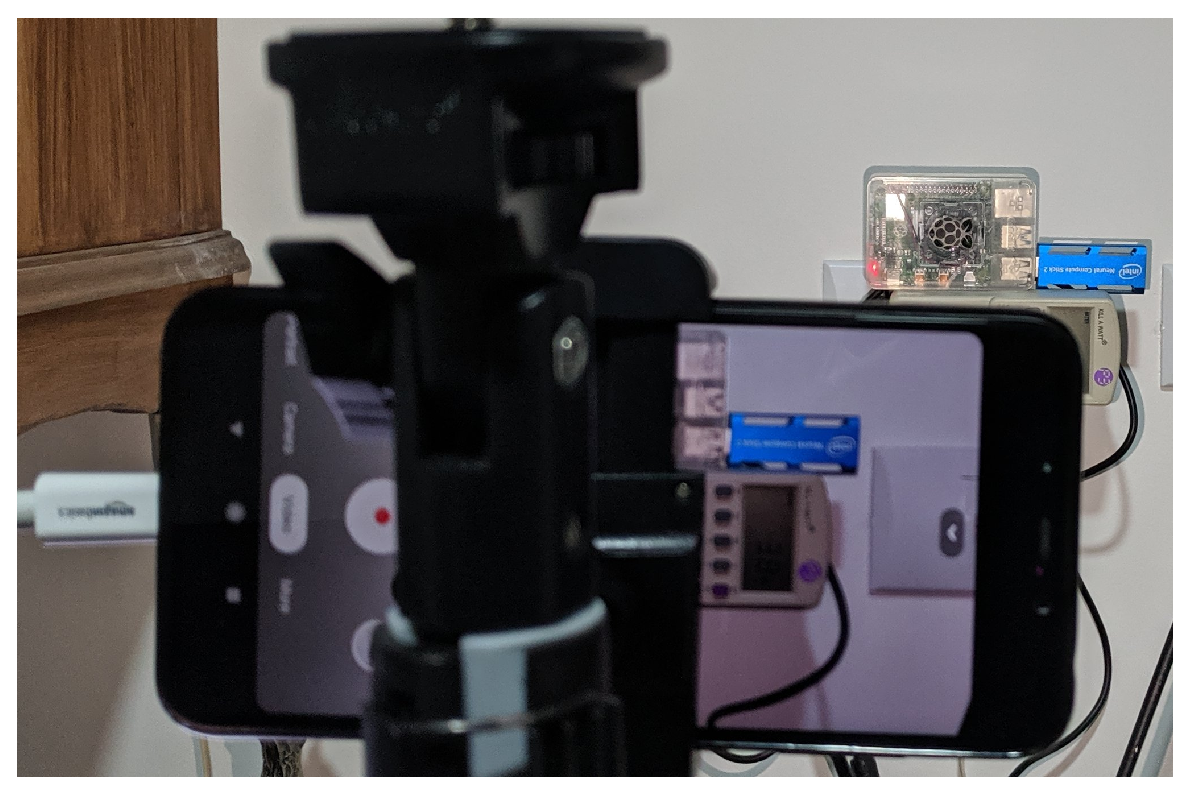
\includegraphics[scale=0.15]{setup2}
	\caption{Test platform. Raspberry Pi 4 with NCS2 attached. Cell phone camera recording power consumption.}
	\label{fig:setup2}
\end{figure}

For each of the three applications these three measurements are considered:

\begin{itemize}
    \item \textbf{Accuracy.} The test dataset is used to test the accuracy of the network. It is given by the percentage of correctly predicted classes out of the total images.
    \item \textbf{Performance.} This is measured doing inference on the whole test dataset and measuring how much time it takes to do the inference. Then, the number of images in the dataset is divided by the amount of time it took to run and that gives the performance metric with units of inferences per second.
    \item \textbf{Average power consumption.} This is measured in Watts and is measured using a Kill-A-Watt device attached to the power brick that powers the device under test (see Figure \ref{fig:setup2}). This measures the complete system power. Note: The NCS2 consumes power when idle, so when measurements were done using Tensorflow the NCS2 was removed from the Raspberry Pi.
\end{itemize}

Apart from these, a fourth, derived metric, is going to be analyzed and it is the \textbf{energy efficiency} measured as performance per Watt. This can be obtained by simply dividing the performance metric by the power consumption (see Equation \ref{eq:ee}).

\begin{equation}\label{eq:ee}
EE = Pe / PC
\qquad (inferences/s/Watt)
\end{equation}

All the mentioned measurements were performed for all the techniques mentioned in the optimizations section above. On top of that, two extra sets of measurements were done: one where all the techniques are combined and another where all the techniques, except for separable convolution, were combined. The reduced input size will reduce the image by 25\%. The reduced CNN depth and layer size will reduce the depth of all the CNNs by 25\% and the amount of neurons in all the fully connected layers by 25\%. For the pruning optimization a pruning target of 50\% is used.

\section{Experimental Evaluation}

\subsection{Accuracy}

Figures \ref{fig:acc-audio}, \ref{fig:acc-fruit} and \ref{fig:acc-scene} show the accuracy achieved by the trained neural networks. These results were measured using the corresponding test dataset. The accuracy was the same for both Tensorflow and OpenVINO.

\begin{figure}[thbp]
	\centering
	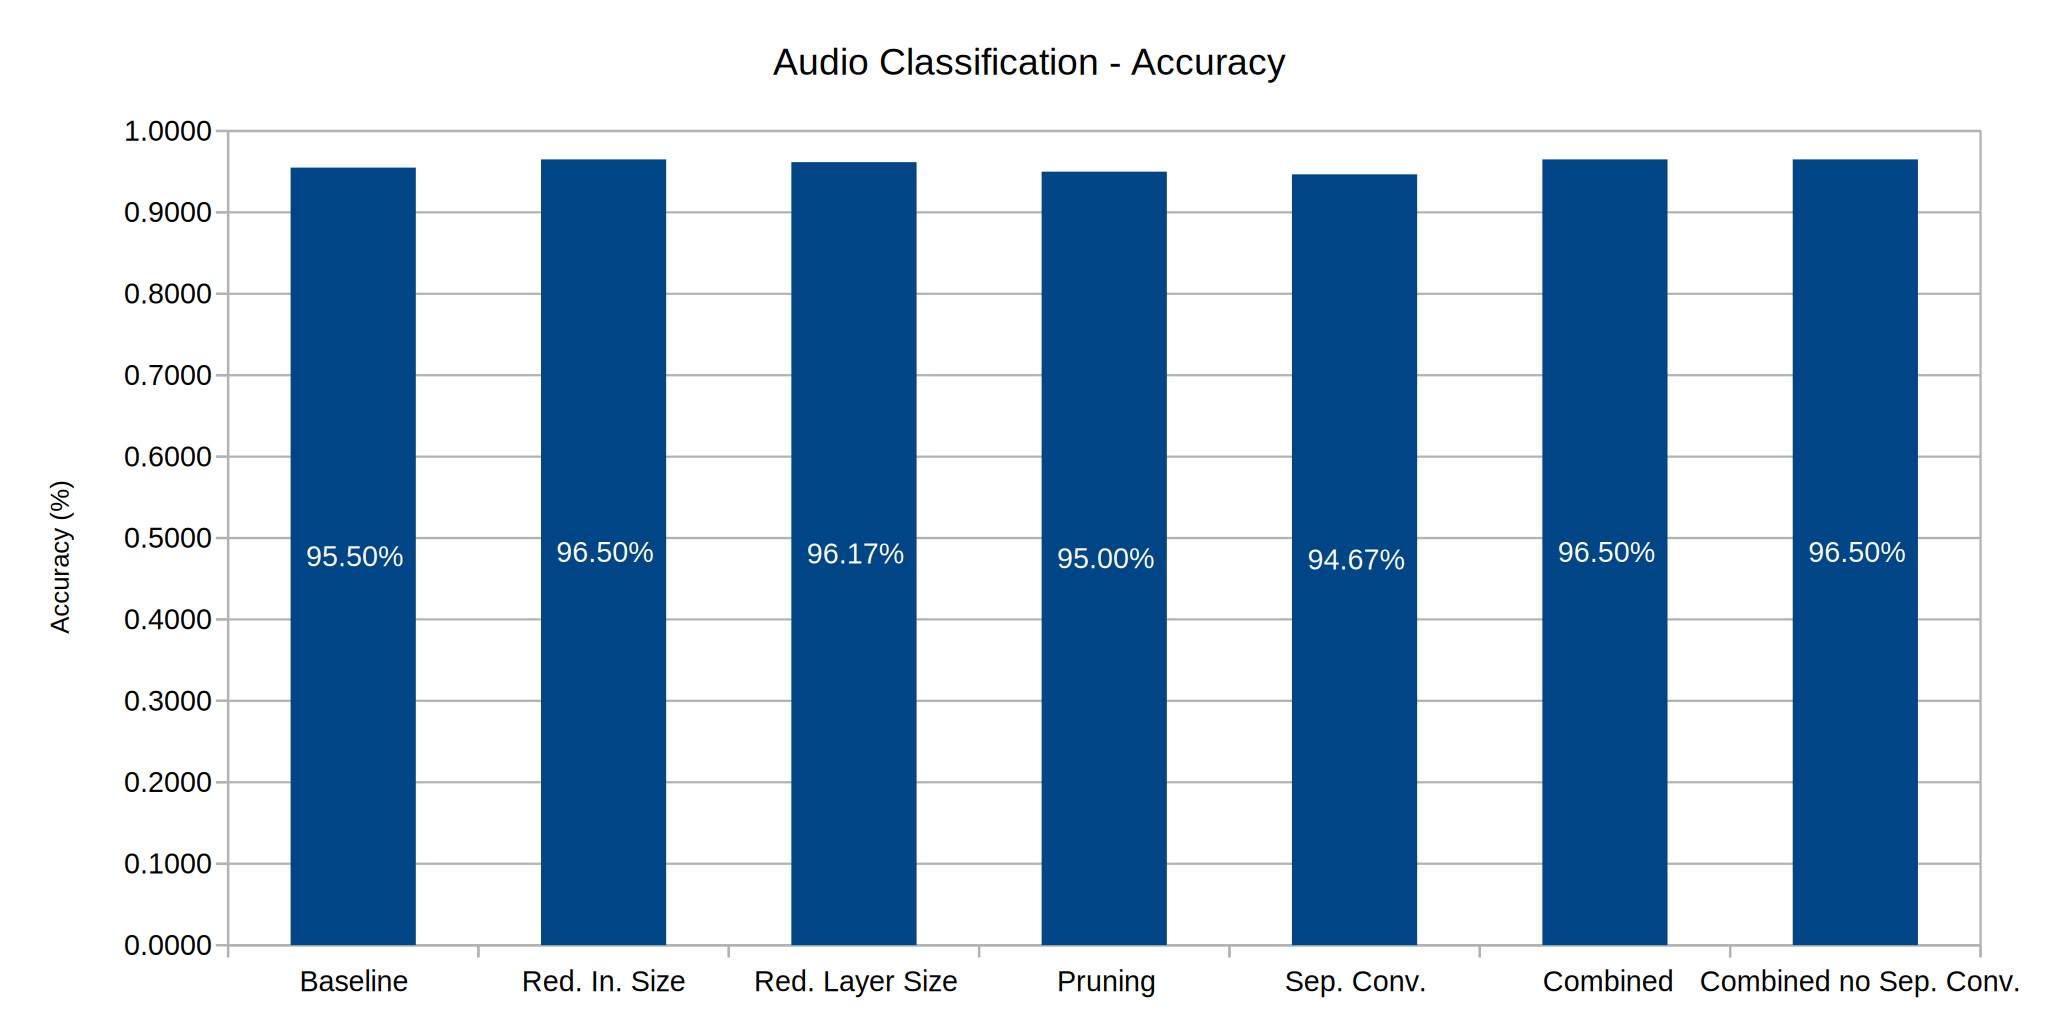
\includegraphics[scale=0.65]{acc-audio}
	\caption{Audio classification: accuracy comparison.}
	\label{fig:acc-audio}
\end{figure}

For the audio classification app the accuracy remains fairly consistent across the different optimizations. Compared to the baseline the worst degradation was seen when running the separable convolution, which reduced the accuracy by 0.83\%. The best case improved the accuracy by 1\%, in the case of the reduced input size and both optimizations with combined techniques.

\begin{figure}[thbp]
	\centering
	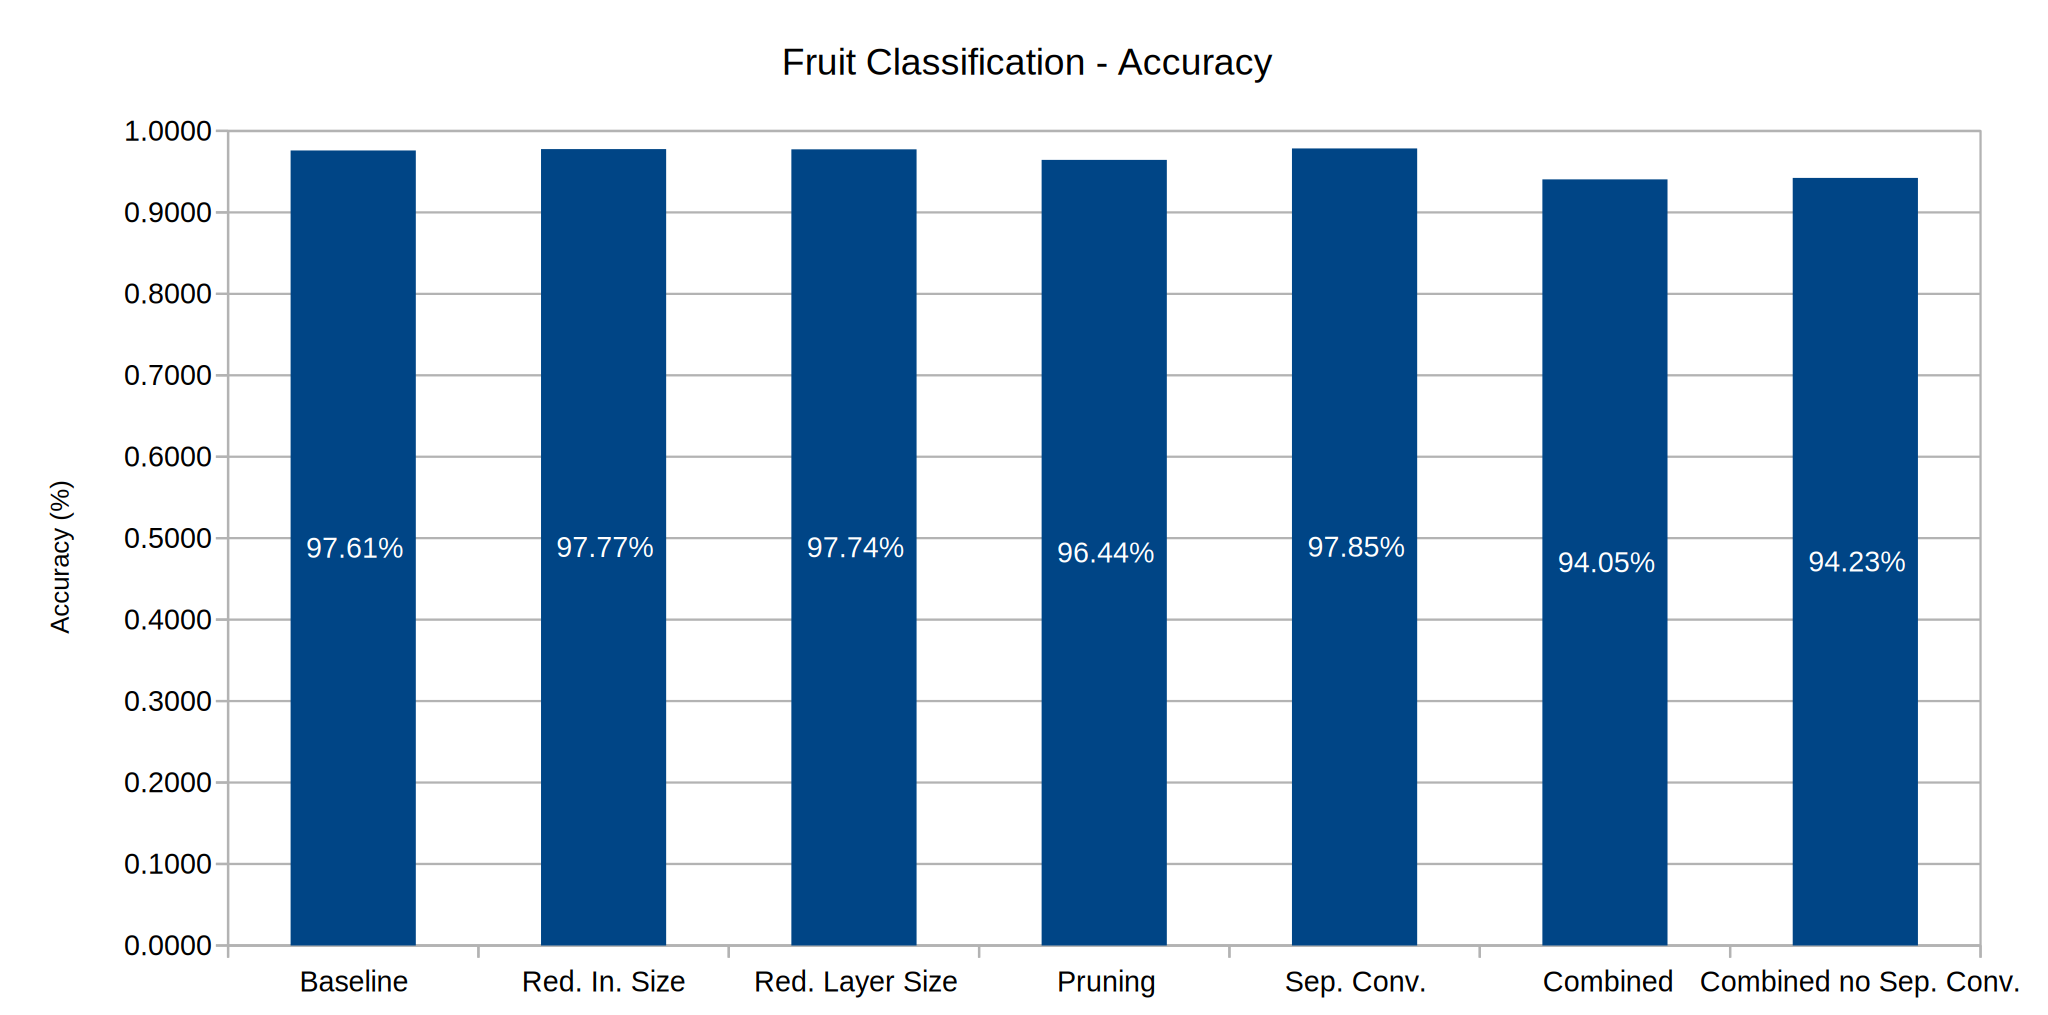
\includegraphics[scale=0.65]{acc-fruit}
	\caption{Fruit classification: accuracy comparison.}
	\label{fig:acc-fruit}
\end{figure}

In the case of the fruit classification the optimization techniques individually didn't have a significant impact in the accuracy. However when combining several techniques together there is a measurable decline in the accuracy. At 94.04\% the accuracy fell by 3.56\%.

\begin{figure}[thbp]
	\centering
	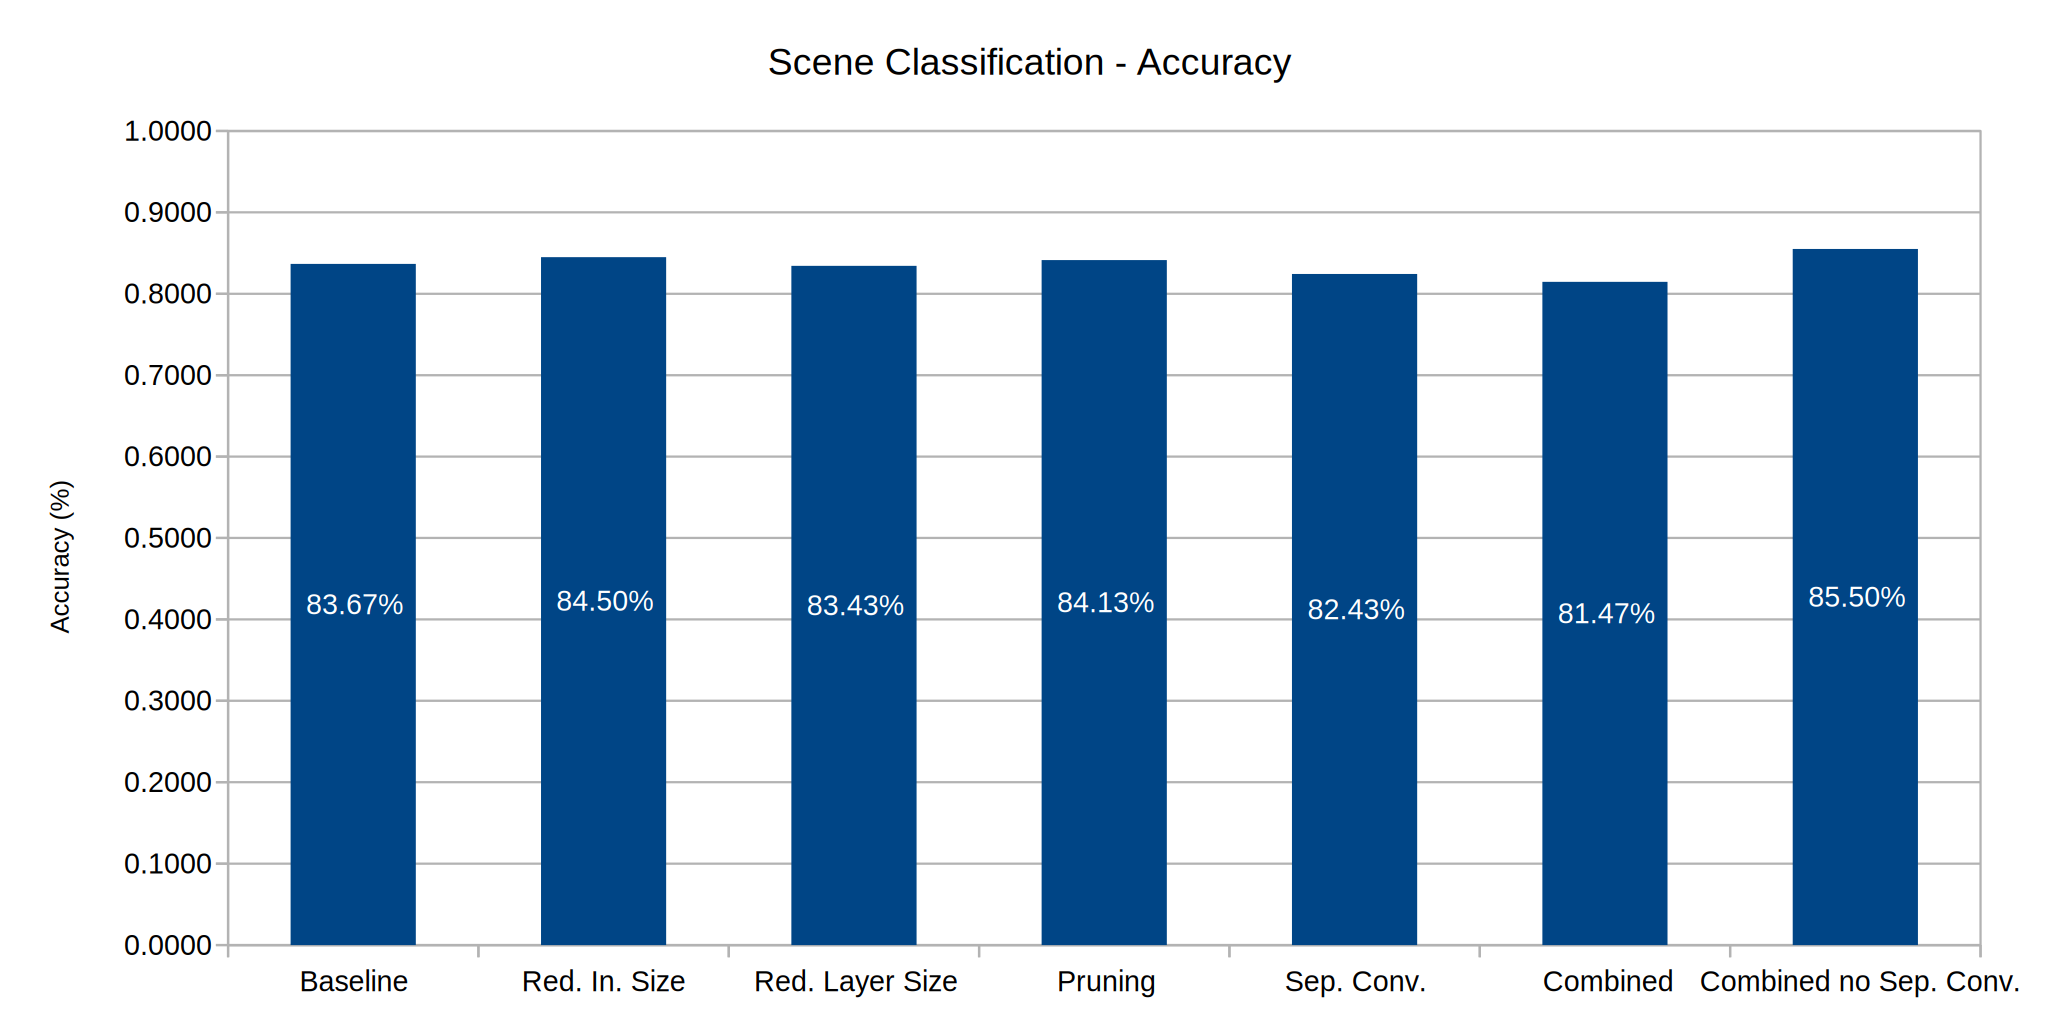
\includegraphics[scale=0.65]{acc-scene}
	\caption{Scene classification: accuracy comparison.}
	\label{fig:acc-scene}
\end{figure}

The scene classification application shows a similar behaviour as the audio classification application. No clear trend is set, which means that the optimization does not really affect the accuracy in a significant way. In fact, when combining all methods except for the separable convolution the accuracy actually improved 1.83\%.

In general, it can be seen that the accuracy is not degraded for the audio and scene classification applications even when combining all the optimizations. The only case where a clear conclusion can be made is in the fruit classification application where the combination of techniques hurts the accuracy by a small percentage.

\subsection{Performance}

Figures \ref{fig:acc-audio}, \ref{fig:acc-fruit} and \ref{fig:acc-scene} show the performance for each of the optimization techniques for both Tensorflow and OpenVINO.

\begin{figure}[thbp]
	\centering
	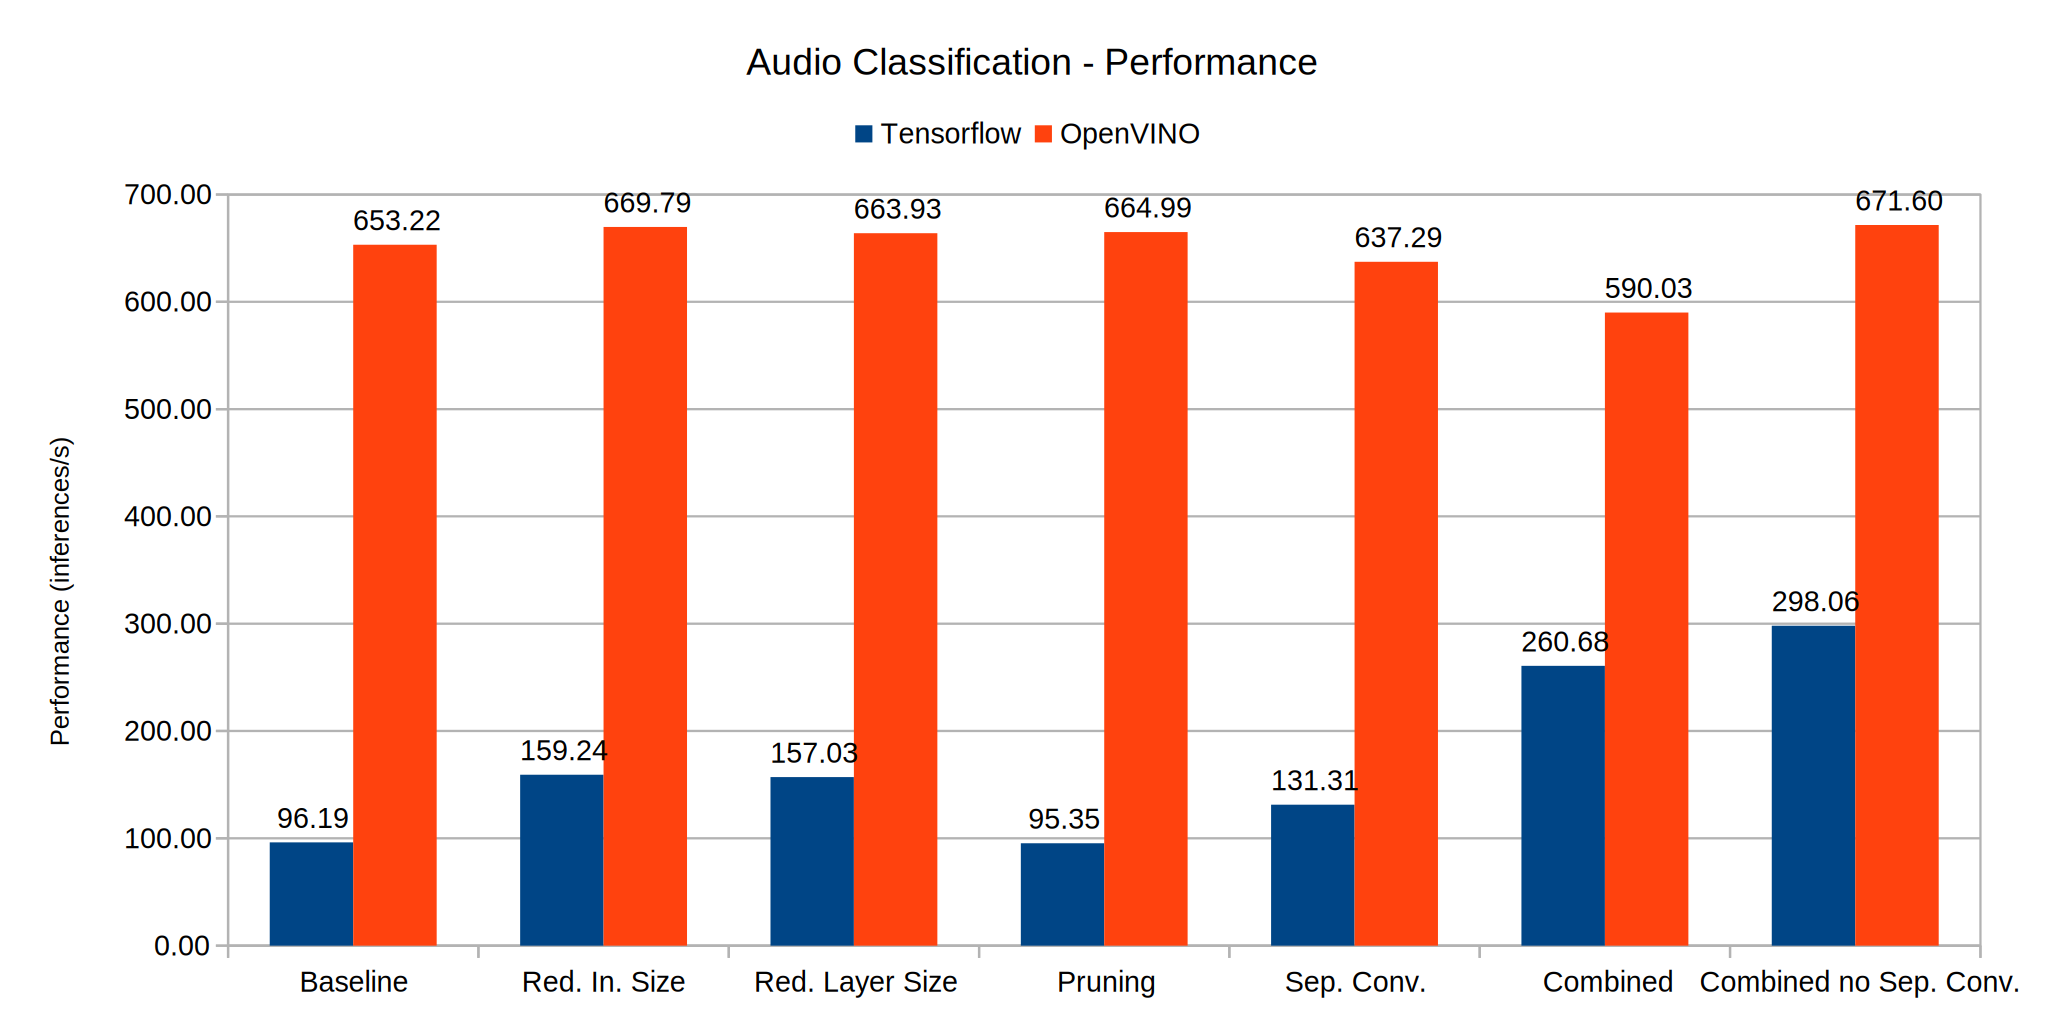
\includegraphics[scale=0.65]{perf-audio}
	\caption{Audio classification: performance comparison.}
	\label{fig:perf-audio}
\end{figure}

Looking at the Tensorflow results for the audio classification application in Figure \ref{fig:acc-audio} all the optimizations except for pruning improved the performance. The best case scenario was achieved by combining all the optimizations except the separable convolution. For that best case the performance improved by 209.9\%. In the case of OpenVINO the best case was also the combined without separable convolution. The difference is that in this case the performance gain was minimal, only an improvement of 2.8\%. Another notable result is that the separable convolution actually hurts performance in this application. In this application OpenVINO was faster than Tensorflow by 125.3\% when comparing the best result for each.

\begin{figure}[thbp]
	\centering
	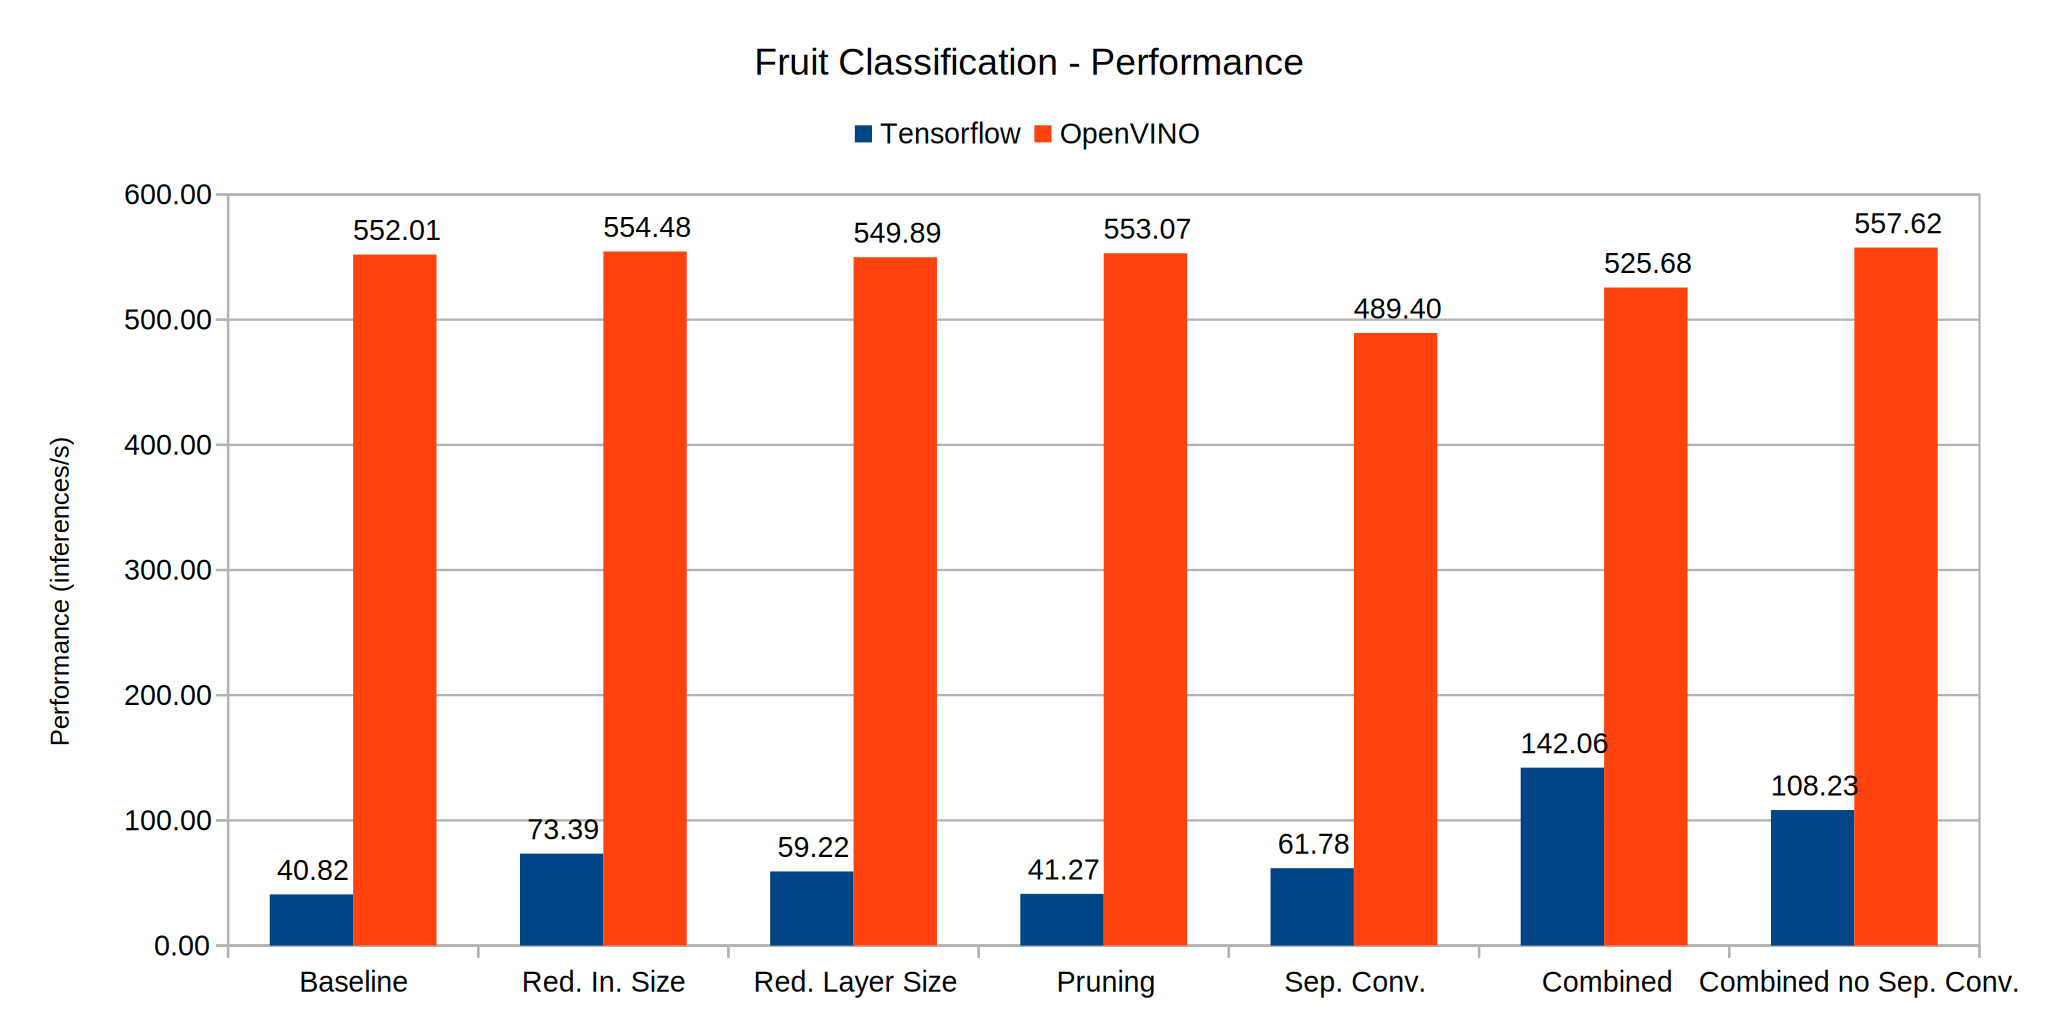
\includegraphics[scale=0.65]{perf-fruit}
	\caption{Fruit classification: performance comparison.}
	\label{fig:perf-fruit}
\end{figure}

The fruit classification application follows a similar trend to the audio classification application (see Figure \ref{fig:acc-fruit}). In this case the difference is that in Tensorflow combining all techniques gives the best performance improvement, which is of 248\%. OpenVINO's trend is the same as for the audio application, where the separable convolution hurts performance so combining all techniques except for it gives the best result. This improvement is very small though, just a 1\%. When the best case for Tensorflow and OpenVINO is compared, it can be seen that OpenVINO is faster by 292.5\%.

\begin{figure}[thbp]
	\centering
	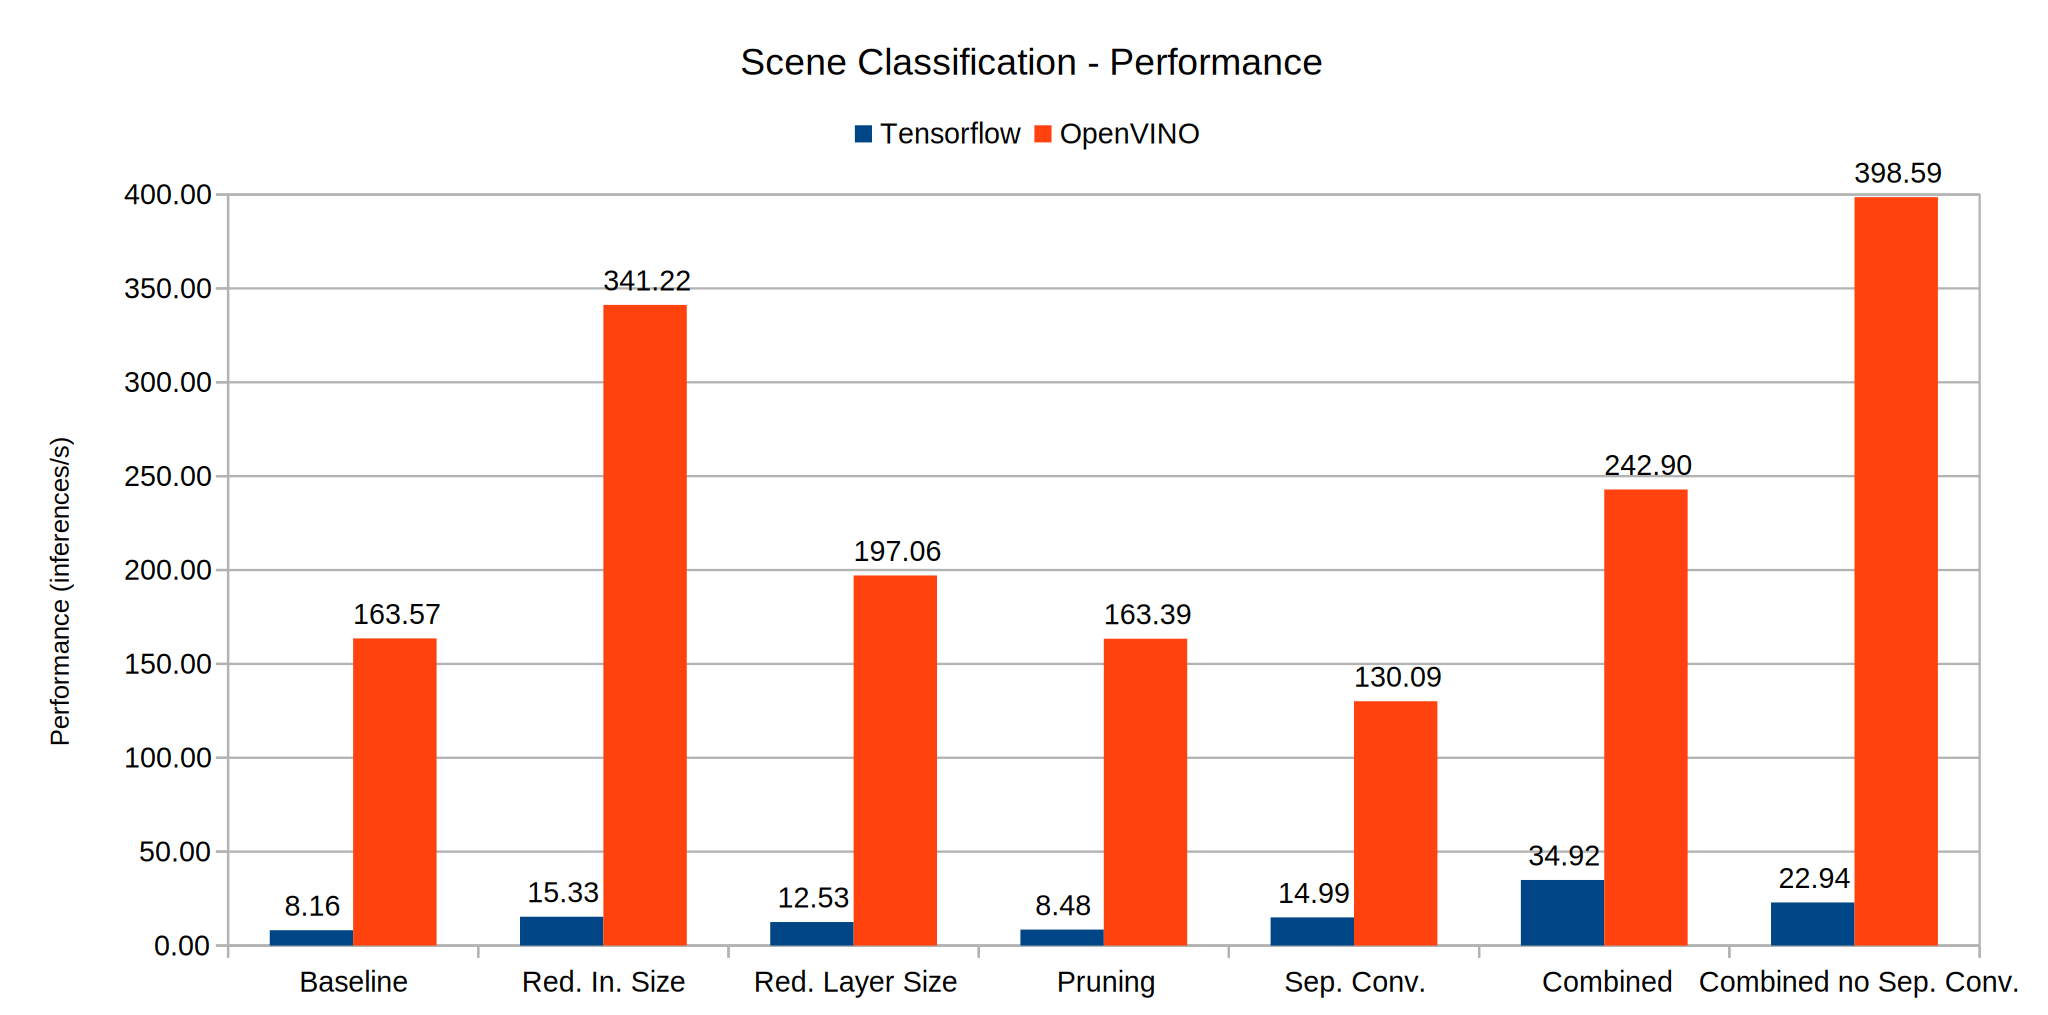
\includegraphics[scale=0.65]{perf-scene}
	\caption{Scene classification: performance comparison.}
	\label{fig:perf-scene}
\end{figure}

In the scene classification application using Tensorflow (see Figure \ref{fig:acc-scene}) the best case achieved was combining all the optimizations, this improved the performance by 328\%. For the case of OpenVINO, this is the only application where a significant improvement can be seen when optimizing the neural network. The best case was again the combination of techniques except for the separable convolution, but this time the improvement was 143.7\%. This application presents the most extreme improvement when comparing Tensorflow and OpenVINO. This time the difference is of 1041.4\%.

This classification problem clearly has a different trend from the other two, the optimizations techniques had a much greater impact on the results. This is the more complex application and as such utilizes a bigger neural network with more than 2 million parameters, compared to 500,000 and 150,000 of the other applications. This means that the Myriad X accelerator spends more of its time doing calculations to execute the network and is not bottle-necked by the data transfer from and to the NCS2. The neural networks of the first two applications are too small and execute so fast that the real impact of the optimization techniques cannot be seen because there are other bottle-necks in the system that hide the optimizations.

In general, a clear trend can be seen where Tensorflow can get significant performance improvements when applying the optimizations but with OpenVINO it varies greatly depending on the application. Another clear result is that the separable convolution optimization doesn't work well with OpenVINO and the NCS2 to the point where it actually hurts performance. In contrast the separable convolution did help when running the applications with Tensorflow. When comparing Tensorflow with respect to OpenVINO it is clear that significant gains in performance can be obtained when running the neural networks in a specialized accelerator such as the Myriad X VPU, applications can run up to 10 times faster when using an optimized toolkit and hardware. The only optimization that didn't affect the results was pruning. This indicates that neither Tensorflow nor OpenVINO are optimized to take advantage of this technique and it is not worth using it.

\subsection{Accuracy vs Performance}

In this section a comparison is made between the accuracy and the performance of the different optimizations. The best results are the ones towards the top right corner, where both the accuracy and performance are maximized. Note that even though the difference between the worst and best case may be small, the graphs are zoomed to fit the data and the difference may seem bigger than they are. This is shown for the OpenVINO scenario.

\begin{figure}[thbp]
	\centering
	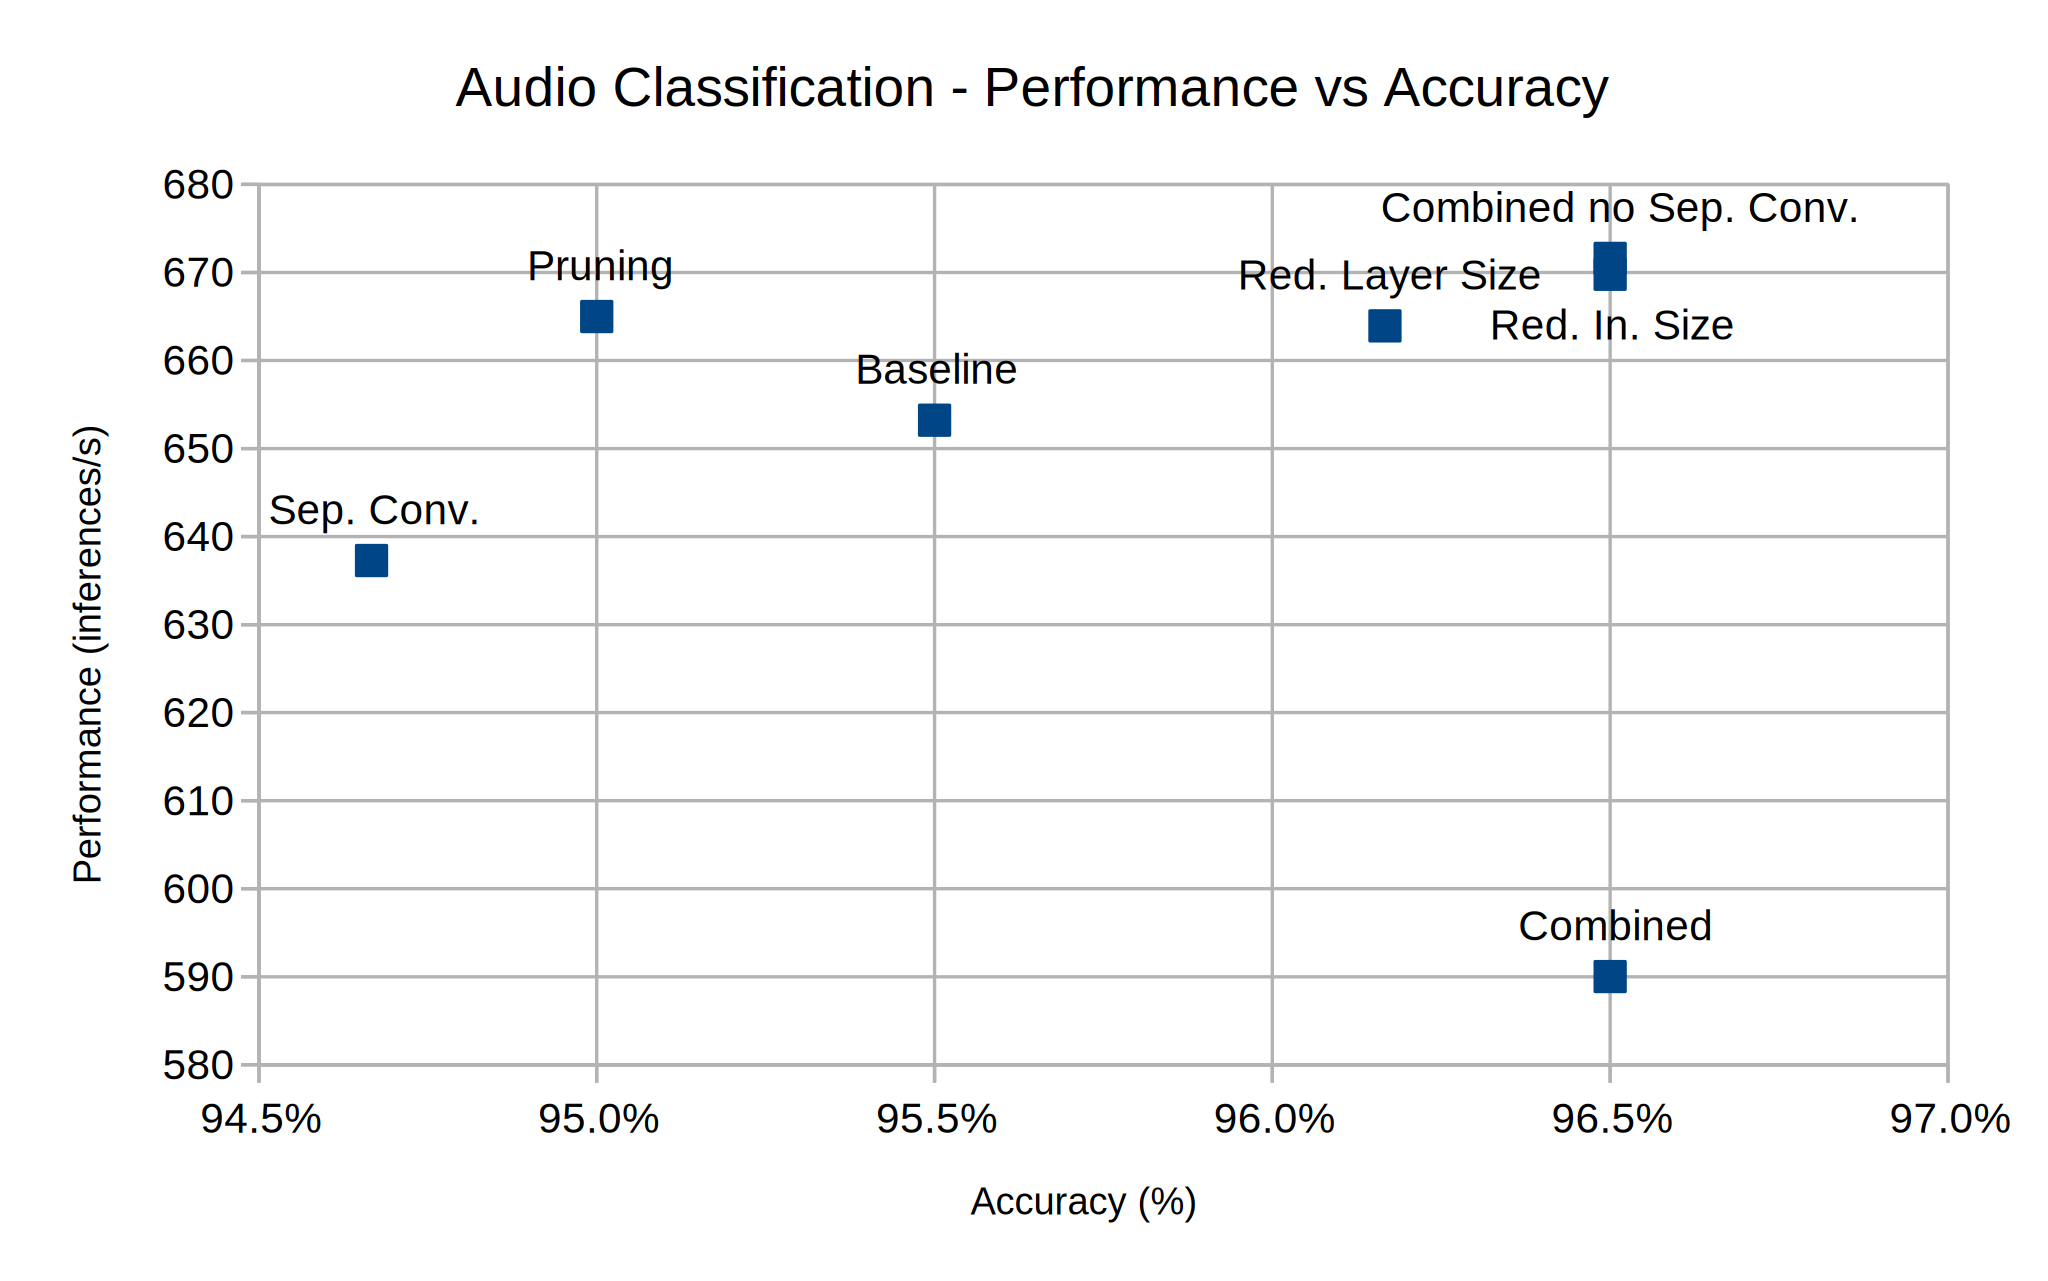
\includegraphics[scale=0.75]{vs-audio}
	\caption{Audio classification: accuracy vs performance.}
	\label{fig:vs-audio}
\end{figure}

In Figure \ref{fig:vs-audio} the results from the audio classification application are shown. The clear winners here are the reduce input size optimization and the case where all optimizations except for the separable convolution are applied. Both have an accuracy of 96.5\% and the performance is nearly identical. This means that reducing the input size of the image is enough optimization to improve the performance without hurting the accuracy.

\begin{figure}[thbp]
	\centering
	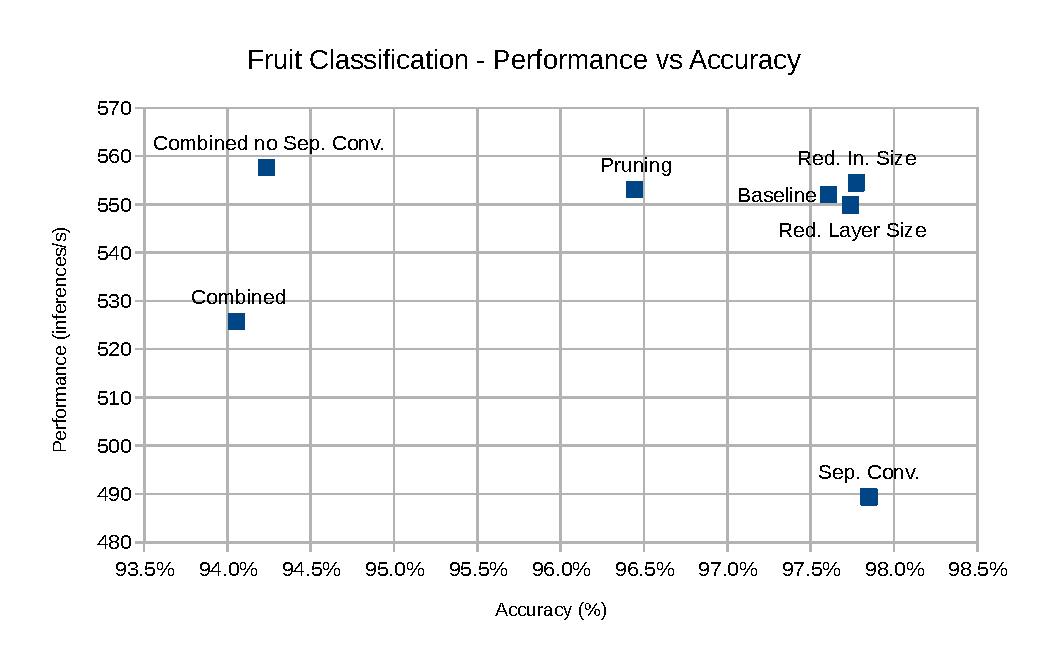
\includegraphics[scale=0.75]{vs-fruit}
	\caption{Fruit classification: accuracy vs performance.}
	\label{fig:vs-fruit}
\end{figure}

Figure \ref{fig:vs-fruit} shows the results for the fruit classification application. For this application the performance improvements are minimal, the best results range between 550 to 560 inferences per second. In this case there are three results clustered in the top right corner. Since the difference between them is so small running the optimizations in this application is almost insignificant when running it in OpenVINO and the baseline application can be run without losing performance or accuracy.

\begin{figure}[thbp]
	\centering
	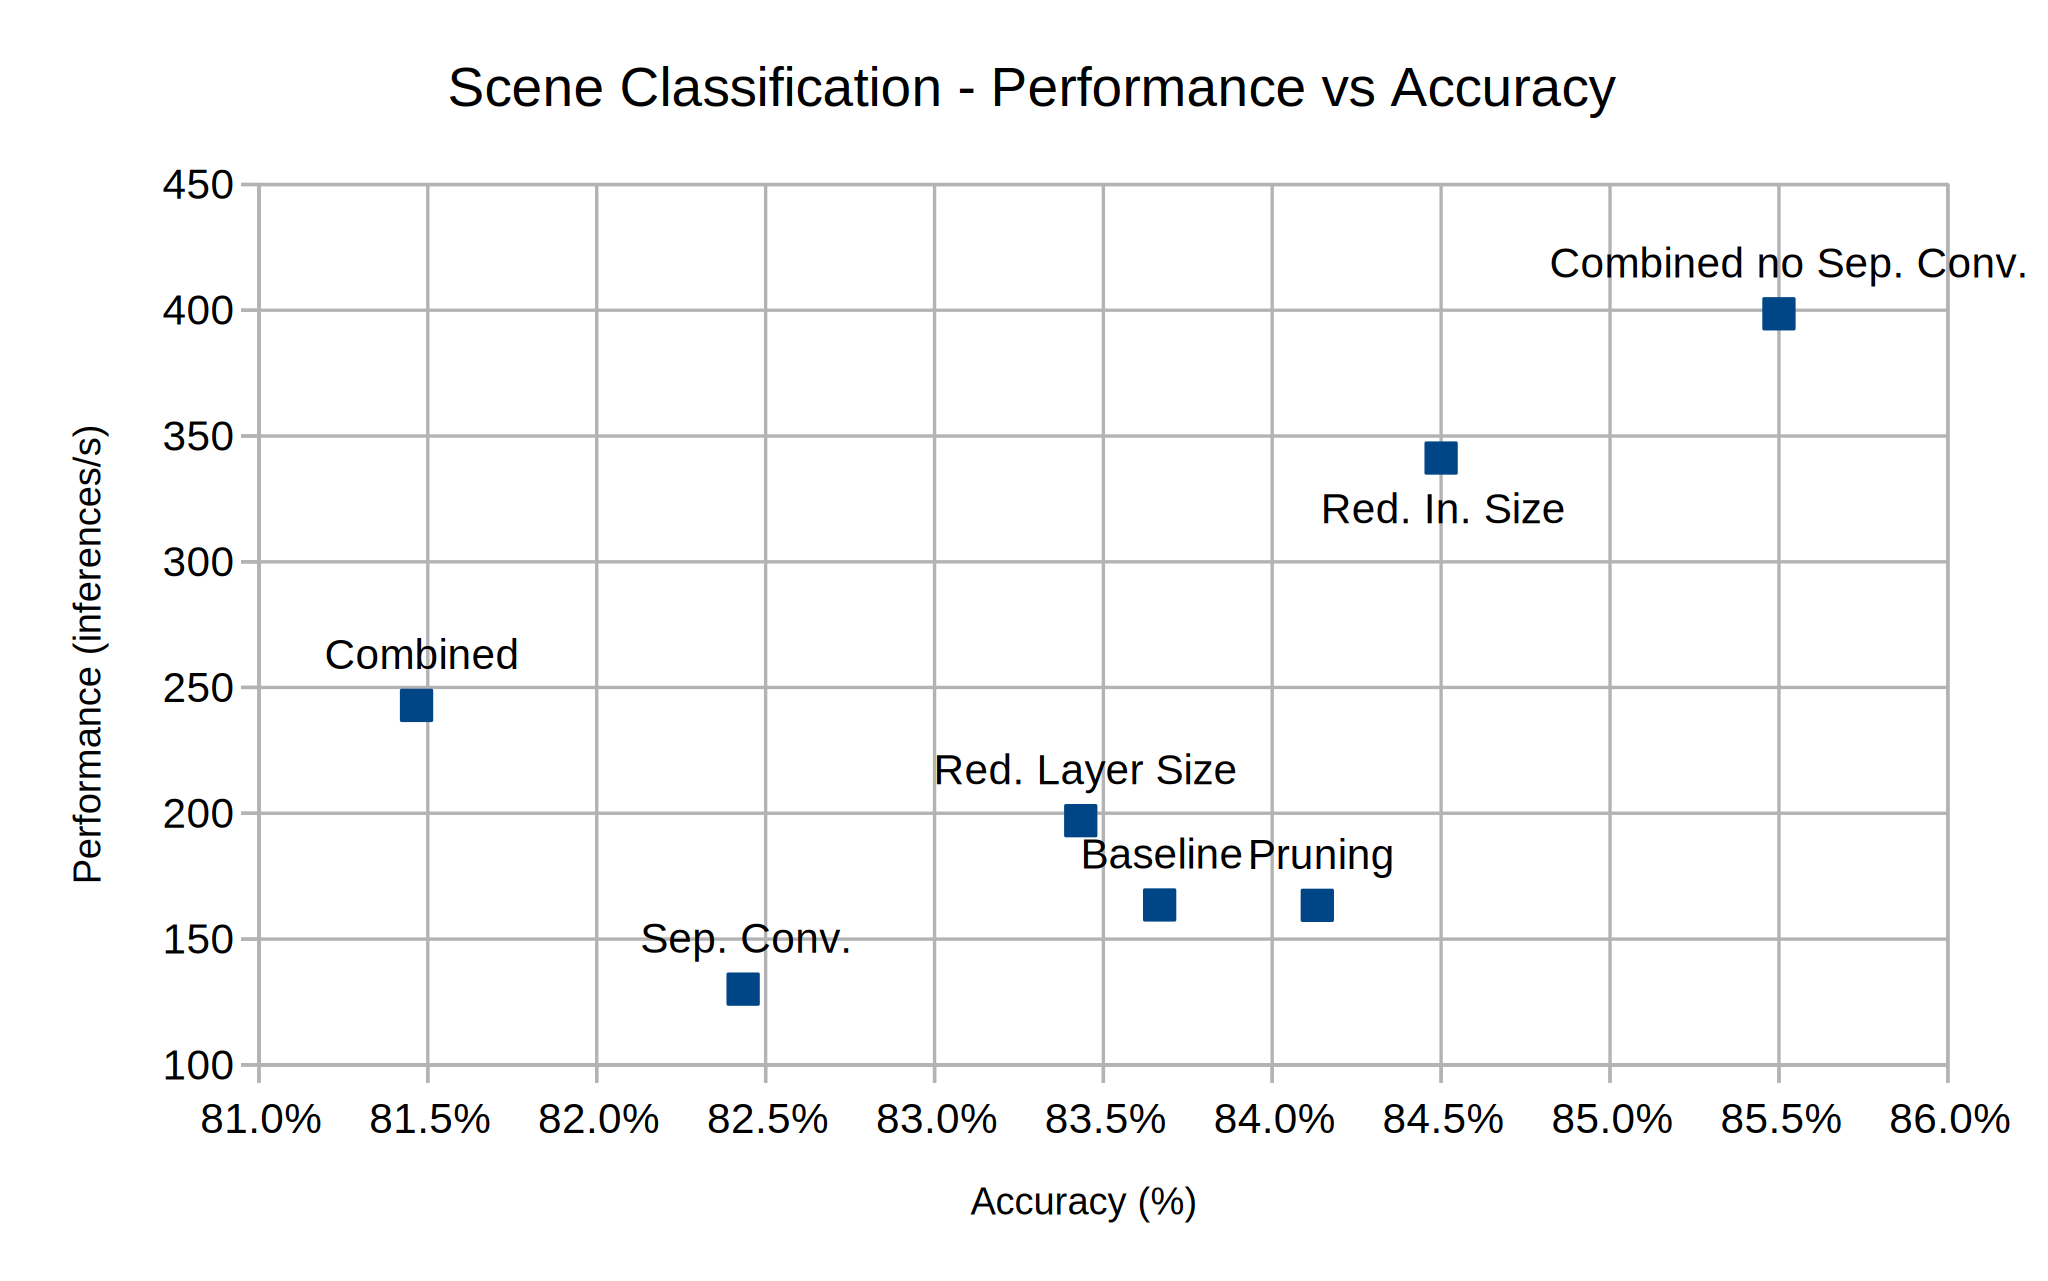
\includegraphics[scale=0.75]{vs-scene}
	\caption{Scene classification: accuracy vs performance.}
	\label{fig:vs-scene}
\end{figure}

For the scene classification application (shown in Figure \ref{fig:vs-scene}) there is a clear winner: combining all the optimization except for the separable convolution. Not only does it have the best performance, it also has the best accuracy. This time the performance is significant (2.43 times faster) unlike the other applications where the performance difference was almost insignificant, only improving by 1 to 3 percent.

\subsection{Power Consumption and Energy Efficiency}

When each of the applications were running the power consumption was logged and a final metric of the average power consumption was calculated, this is measured in Watts. The energy efficiency is defined as the performance per Watt, this is calculated by dividing the performance by the average power consumption.

\begin{table}[thbp]
\centering
\caption{Average power consumption for the audio classification application.}
\label{tab:eet-audio}
\begin{tabular}{|l|l|l|}
\hline
\multicolumn{1}{|c|}{\multirow{2}{*}{\textbf{Optimization}}} & \multicolumn{2}{c|}{\textbf{Power (W)}}                                           \\ \cline{2-3} 
\multicolumn{1}{|c|}{}                                       & \multicolumn{1}{c|}{\textbf{Tensorflow}} & \multicolumn{1}{c|}{\textbf{OpenVINO}} \\ \hline
Baseline                                                     & 5.9                 & 6.2               \\ \hline
Reduced Input Size                                           & 6.0                 & 6.0               \\ \hline
Reduced Layers Size                                          & 6.1                 & 6.1               \\ \hline
Pruning                                                      & 5.9                 & 6.1               \\ \hline
Separable Convolution                                        & 5.4                 & 6.2               \\ \hline
Combined                                                     & 5.0                 & 5.9               \\ \hline
Combined without Separable Convolution                       & 5.9                 & 6.0               \\ \hline
\end{tabular}
\end{table}

\begin{figure}[thbp]
	\centering
	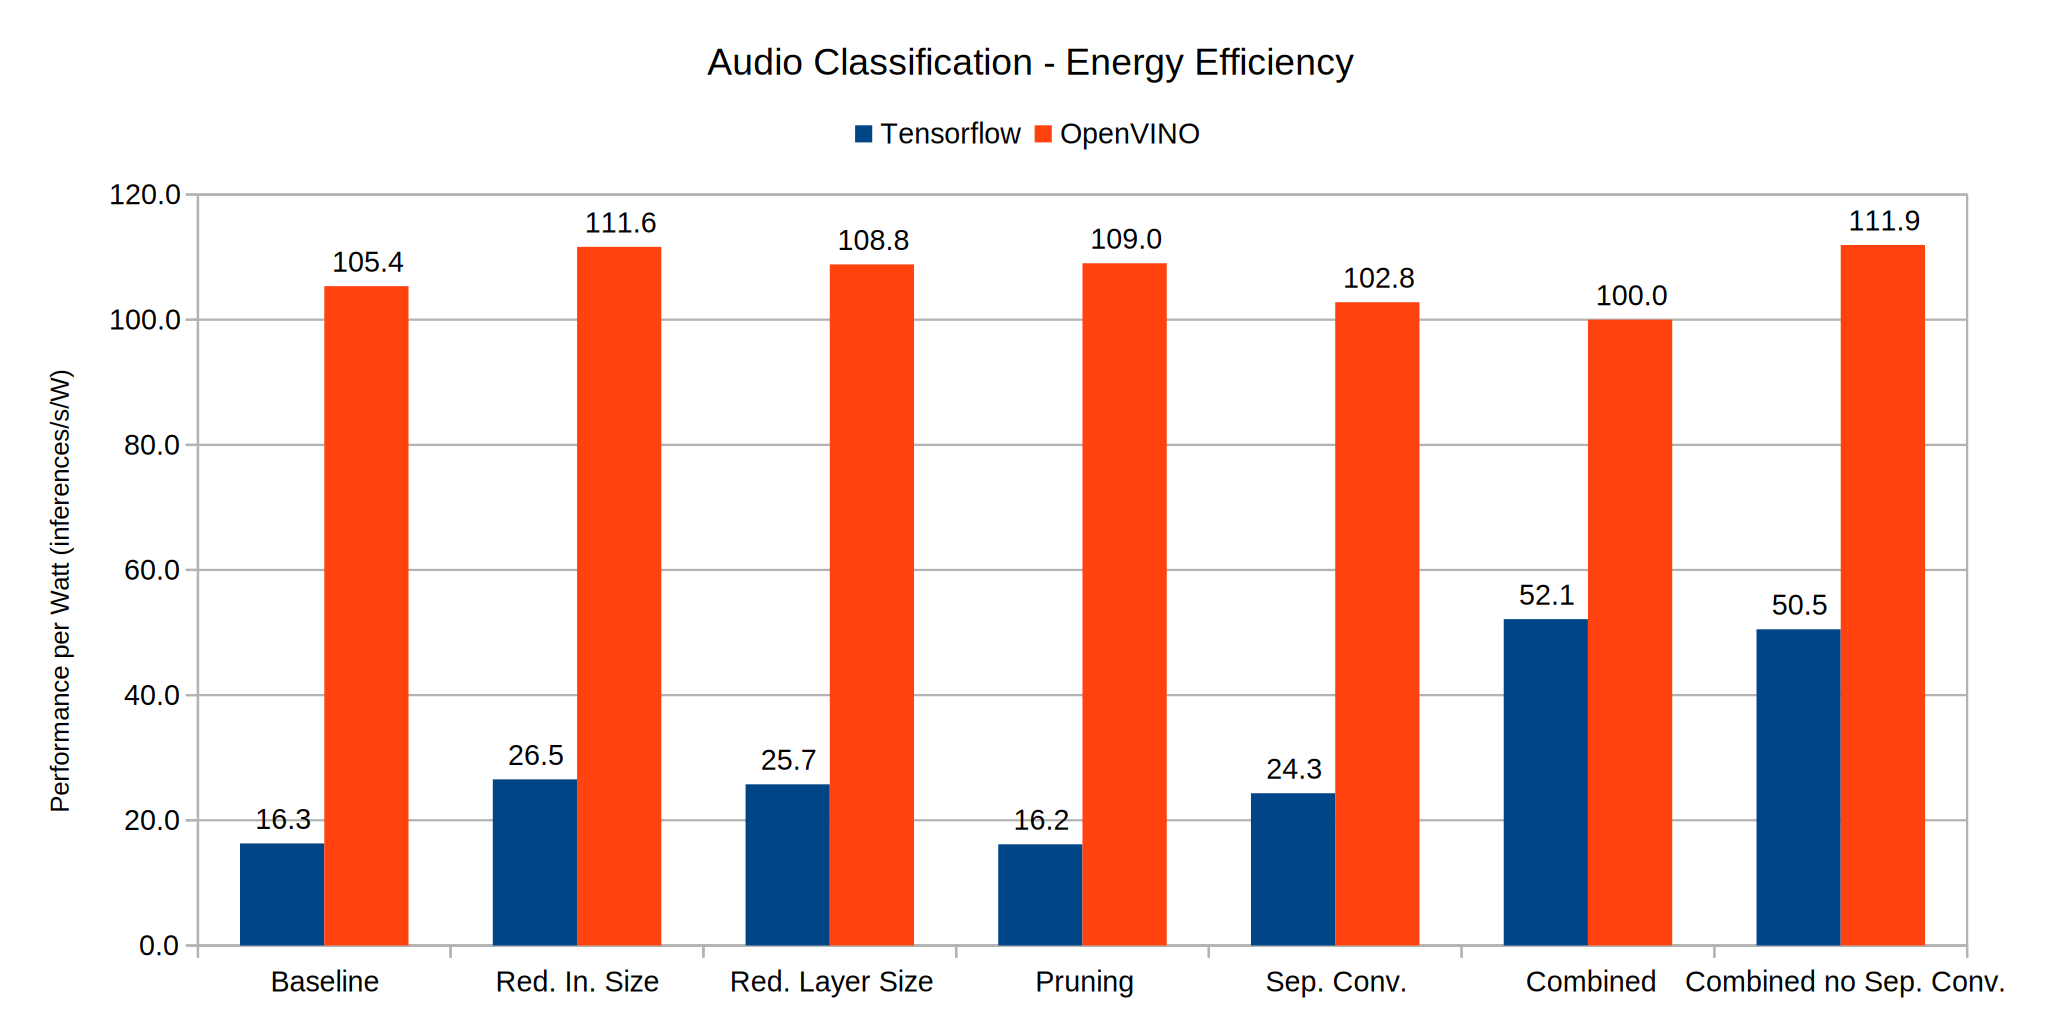
\includegraphics[scale=0.65]{ee-audio}
	\caption{Audio classification: energy efficiency comparison.}
	\label{fig:ee-audio}
\end{figure}

For the audio classification application Table \ref{tab:eet-audio} shows the power consumption metrics for each of the optimizations and Figure \ref{fig:ee-audio} shows the energy efficiency. The power consumption hovers around 6 Watts for most cases except for the separable convolution and the combined case when running with Tensorflow. When looking at the energy efficiency it follows a very similar trend as the performance chart at Figure \ref{fig:perf-audio}. Since the power consumption is so similar between all the cases this is expected. Overall OpenVINO consumes about the same power to run the application but runs much faster which makes it more energy efficient than Tensorflow, comparing the best cases for both OpenVINO has 2.15 times more performance per Watt.

\begin{table}[thbp]
\centering
\caption{Average power consumption for the fruit classification application.}
\label{tab:eet-fruit}
\begin{tabular}{|l|l|l|}
\hline
\multicolumn{1}{|c|}{\multirow{2}{*}{\textbf{Optimization}}} & \multicolumn{2}{c|}{\textbf{Power (W)}}                                           \\ \cline{2-3} 
\multicolumn{1}{|c|}{}                                       & \multicolumn{1}{c|}{\textbf{Tensorflow}} & \multicolumn{1}{c|}{\textbf{OpenVINO}} \\ \hline
Baseline                                                     & 6.1                 & 6.1               \\ \hline
Reduced Input Size                                           & 6.0                 & 6.3               \\ \hline
Reduced Layers Size                                          & 6.2                 & 6.3               \\ \hline
Pruning                                                      & 6.2                 & 6.4               \\ \hline
Separable Convolution                                        & 5.2                 & 6.0               \\ \hline
Combined                                                     & 5.2                 & 6.0               \\ \hline
Combined without Separable Convolution                       & 6.0                 & 5.9               \\ \hline
\end{tabular}
\end{table}

\begin{figure}[thbp]
	\centering
	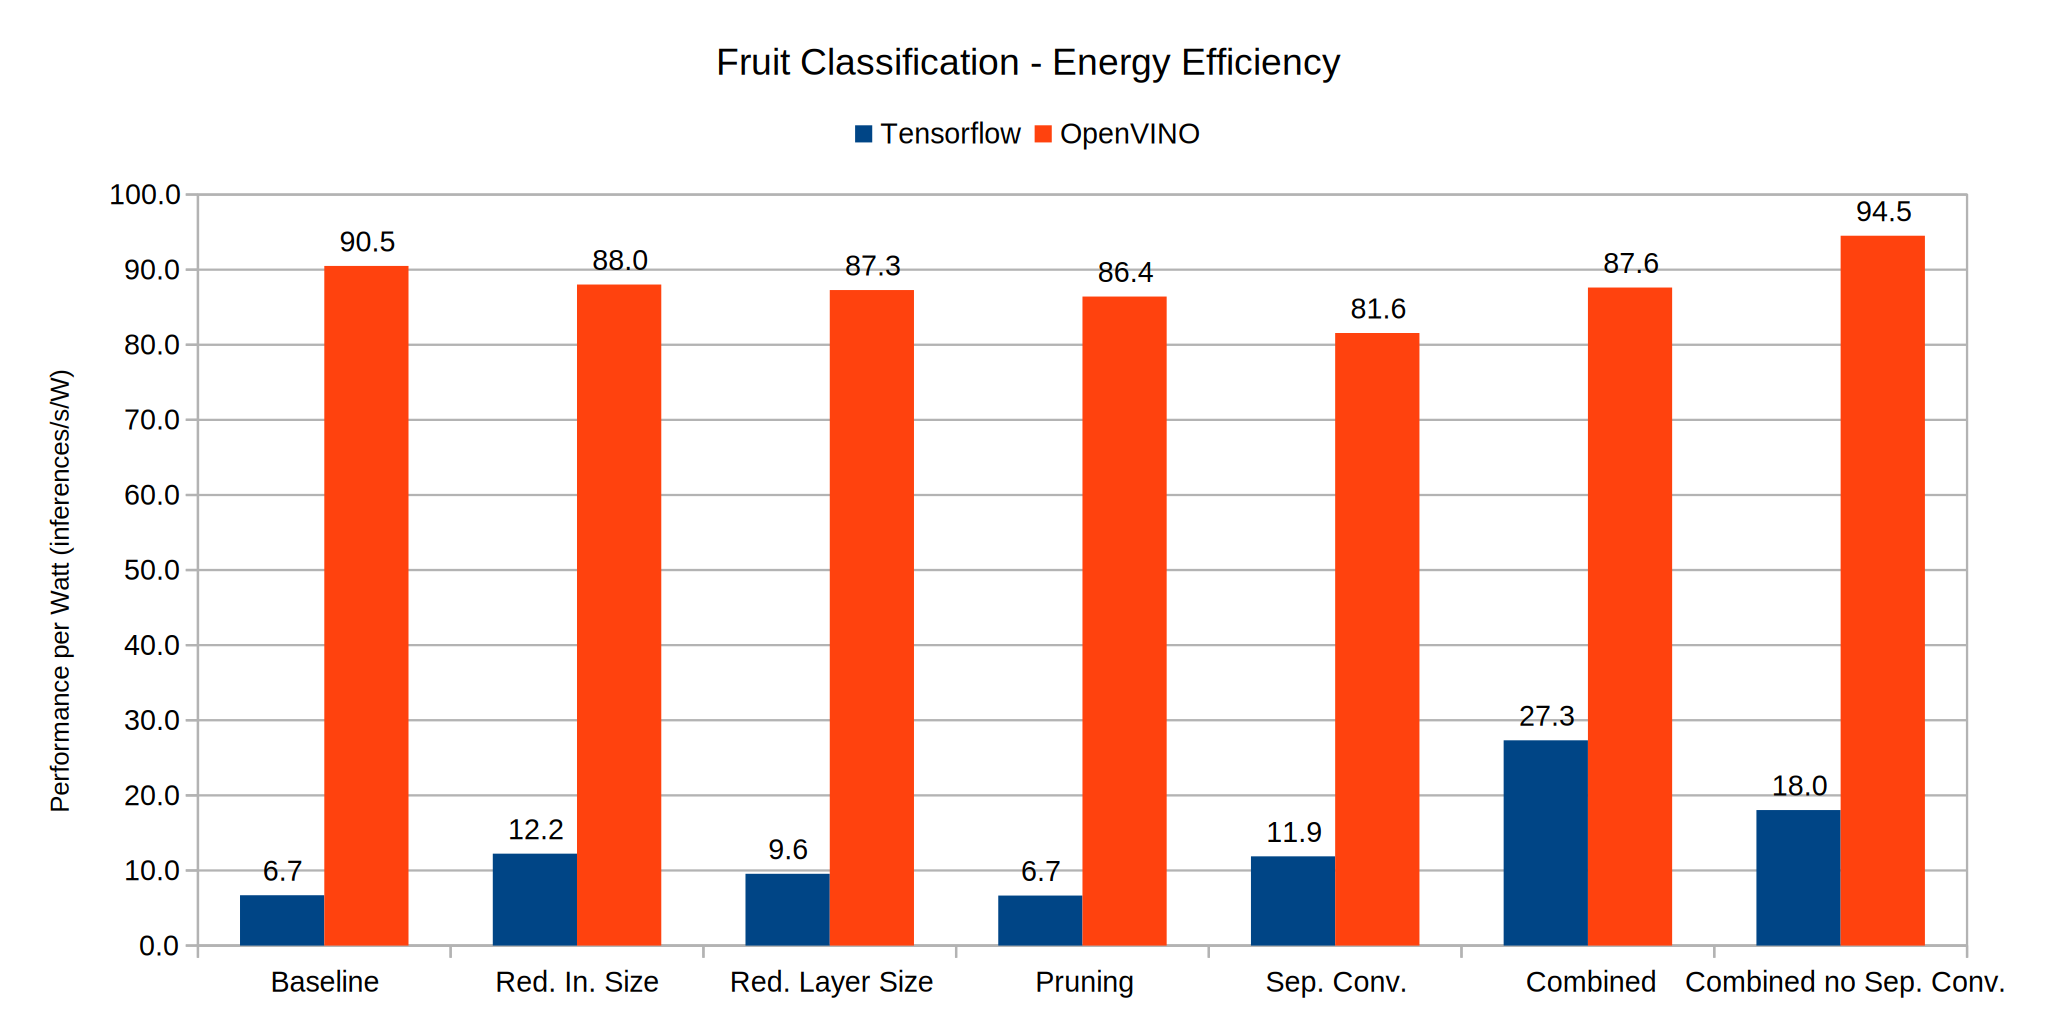
\includegraphics[scale=0.65]{ee-fruit}
	\caption{Fruit classification: energy efficiency comparison.}
	\label{fig:ee-fruit}
\end{figure}

The fruit classification application behaves very similar to the audio classification application. Table \ref{tab:eet-fruit} shows that the power consumption hovers between 6 and 6.4 Watts except when the separable convolution is used in Tensorflow. The performance per Watt follows the same trend as the audio application, Figure \ref{fig:ee-fruit} shows that when comparing the best case for each toolkit, OpenVINO is 3.46 times more energy efficient.

\begin{table}[thbp]
\centering
\caption{Average power consumption for the scene classification application.}
\label{tab:eet-scene}
\begin{tabular}{|l|l|l|}
\hline
\multicolumn{1}{|c|}{\multirow{2}{*}{\textbf{Optimization}}} & \multicolumn{2}{c|}{\textbf{Power (W)}}                                           \\ \cline{2-3} 
\multicolumn{1}{|c|}{}                                       & \multicolumn{1}{c|}{\textbf{Tensorflow}} & \multicolumn{1}{c|}{\textbf{OpenVINO}} \\ \hline
Baseline                                                     & 6.4                 & 6.2               \\ \hline
Reduced Input Size                                           & 6.4                 & 6.6               \\ \hline
Reduced Layers Size                                          & 6.2                 & 6.2               \\ \hline
Pruning                                                      & 6.2                 & 6.3               \\ \hline
Separable Convolution                                        & 5.4                 & 5.8               \\ \hline
Combined                                                     & 5.5                 & 5.7               \\ \hline
Combined without Separable Convolution                       & 6.4                 & 6.4               \\ \hline
\end{tabular}
\end{table}

\begin{figure}[thbp]
	\centering
	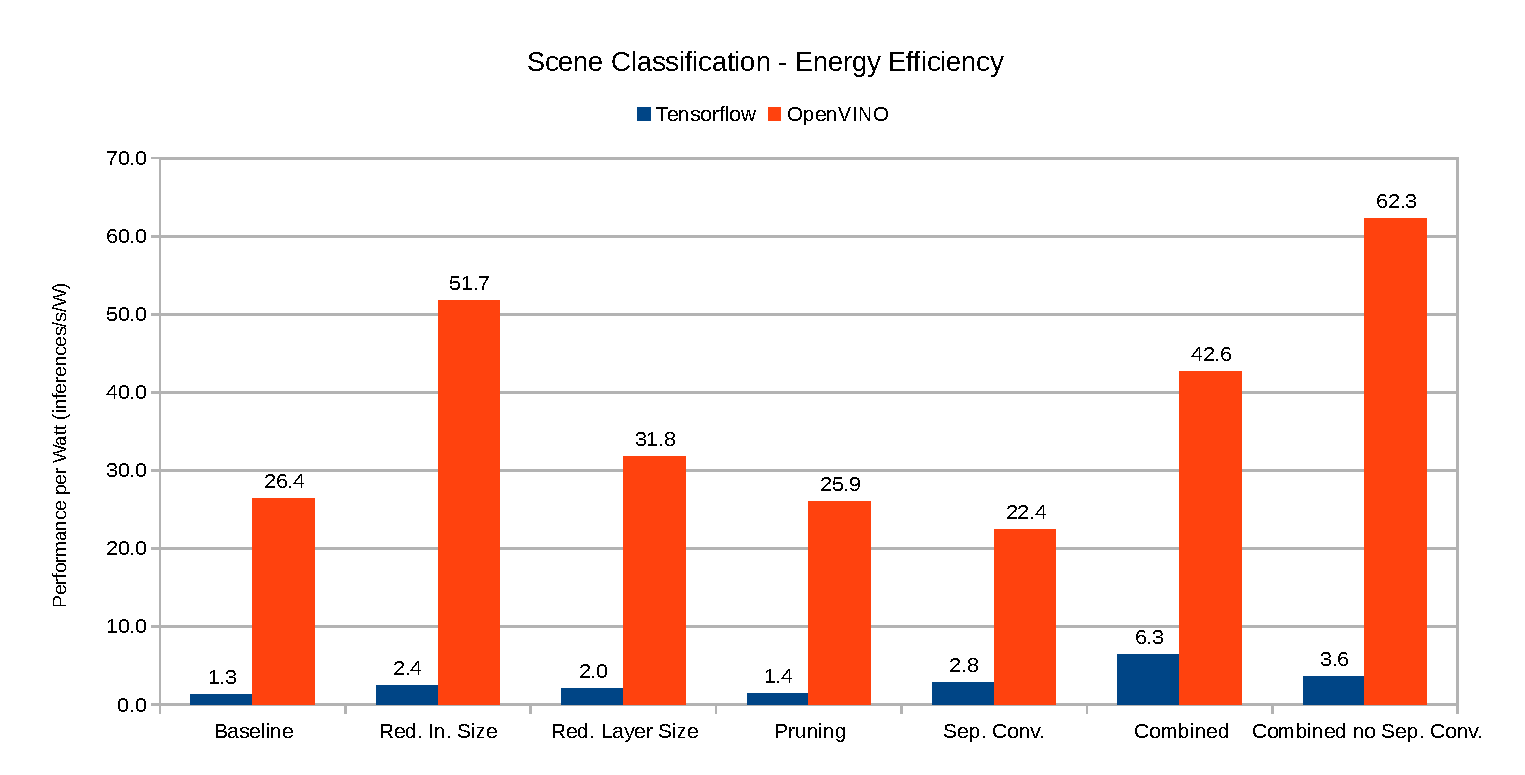
\includegraphics[scale=0.65]{ee-scene}
	\caption{Scene classification: energy efficiency comparison.}
	\label{fig:ee-scene}
\end{figure}

Finally, the scene classification application power consumption results are shown in Table \ref{tab:eet-scene}. This application consumes a little bit more power than the others, it hovers around 6.4 Watts. Similarly to the other applications, when the separable convolution optimization is present the power consumption is lower. This time OpenVINO also shows a reduction in power consumption when the separable convolution is present, something that was not seen in the other applications. Since the performance differences were more drastic the performance per Watt also shows significant differences between the different optimizations. When comparing the best case scenario for each toolkit, OpenVINO comes ahead. It is 9.89 times more energy efficient than Tensorflow.

In general, both Tensorflow and OpenVINO consume about the same amount of power. Since OpenVINO runs much faster this translates into an advantage in energy efficiency measured as performance per Watt.

\section{A Note On Quantization}

% Accuracy.

% \begin{figure}[thbp]
% 	\centering
% 	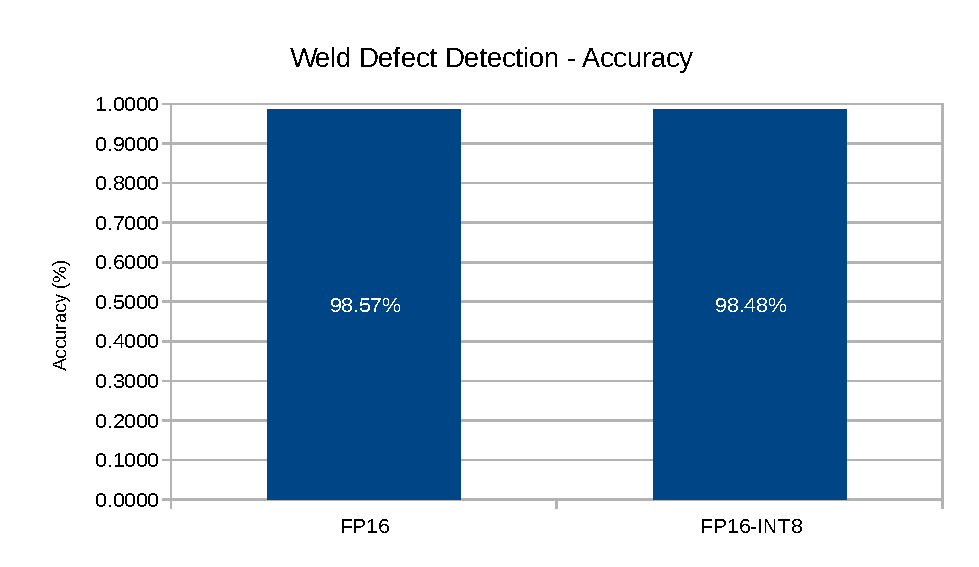
\includegraphics[scale=0.75]{acc-weld}
% 	\caption{Weld defects detection: accuracy comparison.}
% 	\label{fig:acc-weld}
% \end{figure}

% Performance.

% \begin{figure}[thbp]
% 	\centering
% 	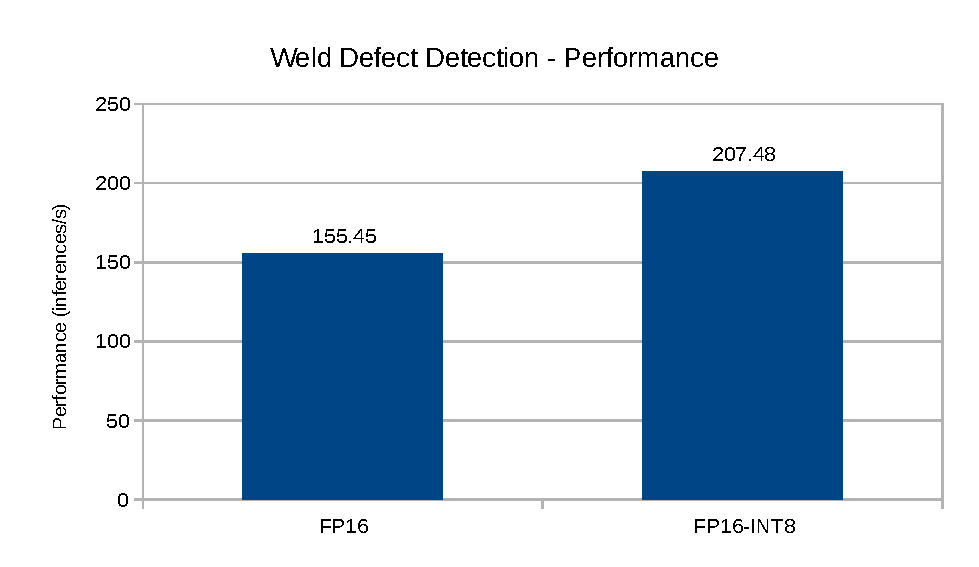
\includegraphics[scale=0.75]{perf-weld}
% 	\caption{Weld defects detection: performance comparison.}
% 	\label{fig:perf-weld}
% \end{figure}

Applying quantization as an optimization technique for neural networks can help performance. This process converts the floating point weights and biases in the layers of the neural network to integer values. In many cases doing integer calculations in hardware can be faster than doing floating point calculations, specially if the hardware supports some kind of SIMD instruction \cite{quant1}. OpenVINO has the capability execution neural networks with INT8 numbers if the hardware supports it \cite{int8}. Unfortunately the NCS2, which uses the Myriad X VPU, doesn't support INT8 operations with OpenVINO \cite{ov_sup_formats}. However most Intel processors support some kind of vector instruction set that can run multiple integer operations in parallel \cite{avx}.

The same desktop PC described in Table \ref{tab:hw_sw_details} was used to test the quantization optimization with OpenVINO. For this test the application selected is a weld porosity detection neural network \cite{weld}. It has three classes: no weld, normal weld and porosity weld. This model is available for download both as a floating point model and as an optimized version where some of the layers are quantized to INT8. The neural network was tested using a private dataset of 10 videos of approximately 20 seconds each.

\begin{figure}[thbp]
	\centering
	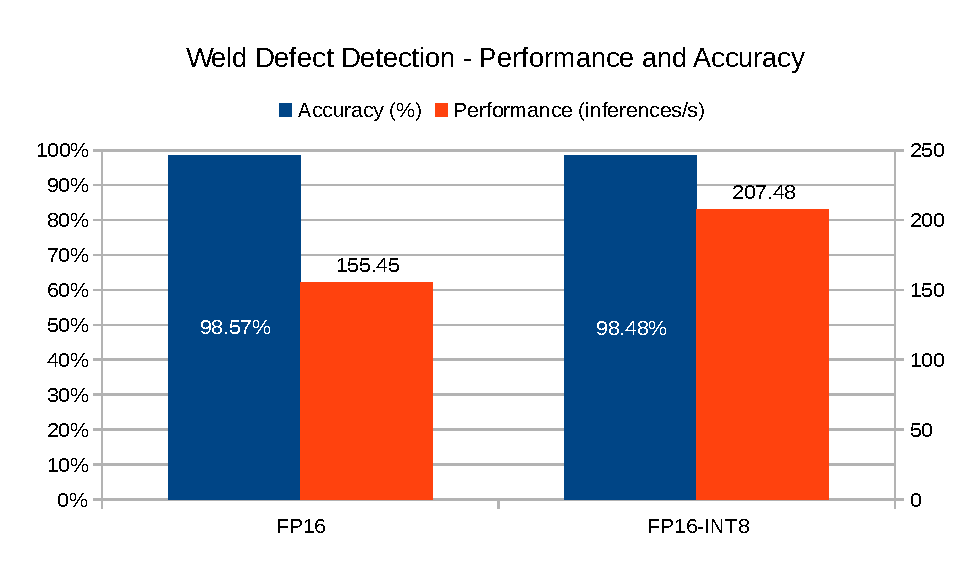
\includegraphics[scale=0.75]{comb-weld}
	\caption{Weld porosity defects detection: accuracy and performance comparison.}
	\label{fig:comb-weld}
\end{figure}

Figure \ref{fig:comb-weld} shows both the accuracy and the performance of the neural network in both cases: floating point and optimized INT8. The results show that the accuracy is barely affected by the quantization. However the performance was increased by 33.5\%.
